\documentclass[12pt]{report}
\usepackage[utf8]{inputenc}
\usepackage{graphicx}
\usepackage{hyperref}
\usepackage{amsmath}
\usepackage{enumitem}
\usepackage{amssymb}
\usepackage{fancyhdr}
\usepackage{multirow}
\usepackage{longtable}
\usepackage{subcaption}
\usepackage{float}
\usepackage[normalem]{ulem}
\graphicspath{ {images/} }
\pagestyle{fancy}
\fancyhf{}
\setlength{\headheight}{15pt}
\lhead{\rmfamily \small \nouppercase \leftmark}
\rfoot{\thepage}
\lfoot{\rmfamily \small \nouppercase \rightmark}
\renewcommand{\headrulewidth}{2pt}
\renewcommand{\footrulewidth}{1pt}
\DeclareMathOperator*{\rint}{\ThisStyle{\hstretch{1.3}{\rotatebox{18}{$\SavedStyle\!\int\!$}}}}
% \usepackage{biblatex}
\usepackage[backend=biber,sorting=none,style=phys,%
articletitle=false,biblabel=brackets,%
chaptertitle=false,pageranges=false]{biblatex}
\addbibresource{thesisbib.bib}
\usepackage[usenames,dvipsnames,x11names]{xcolor}
\usepackage{tikz}
\usetikzlibrary{arrows,shapes,decorations.pathmorphing,positioning,chains}
% Set up a few colours
\colorlet{lcfree}{Green3}
\colorlet{lcnorm}{Blue3}
\colorlet{lccong}{Red3}
\addbibresource{./thesisbib.bib}
\pgfdeclarelayer{marx}
\pgfsetlayers{main,marx}
% A macro for marking coordinates (specific to the coordinate naming
% scheme used here). Swap the following 2 definitions to deactivate
% marks.
\providecommand{\cmark}[2][]{%
  \begin{pgfonlayer}{marx}
    \node [nmark,yshift=1em] at (c#2#1) {#2};
  \end{pgfonlayer}{marx}
  } 
\providecommand{\cmark}[2][]{\relax} 
\newcommand{\proton}[1]{%
	\shade[ball color=red] (#1) circle (.25);
}

%\neutron{xposition,yposition}
\newcommand{\neutron}[1]{%
	\shade[ball color=green] (#1) circle (.25);
}
\newcommand{\pion}[1]{%
	\shade[ball color=blue] (#1) circle (.15);
}

%\electron{xwidth,ywidth,rotation angle}
\newcommand{\electron}[3]{%
	\draw[rotate = #3](0,0) ellipse (#1 and #2)[color=blue];
	\shade[ball color=Gold2] (0,#2)[rotate=#3] circle (.1);
}
\newcommand{\nucleust}{%
	\neutron{7.2,-1.3}
	\proton{7,-1}
	\neutron{7.3,-1.2}
	\proton{6.8,-1.1}
	\neutron{6.9,-1.3}
	\proton{7.2,-1.15}
	\neutron{6.95,-1.12}
}

\newcommand{\nucleus}{%
	\neutron{0.2,0.3}
	\proton{0,0}
	\neutron{0.3,0.2}
	\proton{-0.2,0.1}
	\neutron{-0.1,0.3}
	\proton{0.2,-0.15}
	\neutron{-0.05,-0.12}
	\proton{0.17,0.21}
	\neutron{-0.21,0.3}
	\proton{0.27,0.21}
	\neutron{0.21,0.3}
	\proton{0.17,0.31}
}



\begin{document}
\begin{titlepage}
	\begin{center}
		\vspace*{1cm}
		\textbf{\Large Doctoral dissertation}\\[0.5cm]	
		\textbf{Prepared in the Institute of Physics
			of the Jagiellonian University}\\[0.5cm]	
		Submitted to the Faculty of Physics,
		Astronomy and Applied Computer Science
		of the Jagiellonian University

		\vspace{1.0cm}
		{
\includegraphics[scale=0.05]{university.png}}	\\
		\vspace{1.0cm}
		\Large Investigations of mechanisms of particle production in proton-induced nuclear spallation  \\
		\vspace{0.5cm}
		\Large Udai Singh\\
		\vspace{0.5cm}
		\large Supervised by:\\
		prof. dr hab. Krzysztof Pysz\\
		\vspace{0.5cm}
		Co-supervised by:\\
		dr. Sushil Sharma\\
			\vfill
		Cracow 2021
	\end{center}
\end{titlepage}
\tableofcontents
\chapter*{Abstract}

Studies of the selected problems in understanding of nuclear spallation physics are undertaken. Among them are the description of the initial phase of proton - target nucleus collision and proceeding of the intranuclear cascade, isotropic emission of nuclear fragments of very broad mass spectrum, contribution of the nonequlibrium and equilibrium processes to the total production cross-section and its dependence on the isotope isospin, 
variation of the total production cross-section related to the number and ratio of protons and neutrons of the  emitted particle. 
New experimental distributions of the double differential production cross-sections ($d^2\sigma/d\Omega dE$) for $p$,  $d$,  $t$, $\pi^{+}$ and $\pi^{-}$ in the $p+Nb$ reaction 
at 3.5 GeV proton beam energy are provided. They have been measured by High Acceptance DiElectron Spectrometer (HADES) experiment. The measured energy range of hydrogen isotopes 
are significantly extended in comparison to the experimental data available in the literature. The new experimental spectra are confronted with the theoretical prediction of three models of intranuclear cascade - GiBUU, UrQMD, INCL++. Discrepancies
of the experimental and theoretical distributions are noticed  and discussed. Experimental data derived from the literature are used for examination of nuclear mechanisms assigned to the nuclear deexcitation phenomena. The comparative analysis of the four model prediction (ABLA07, GEMINI++, GEM2, SMM) of the selected observables relevant to the isotropic nuclear fragment emission is performed. Disagreement of the model prediction and the experimental data is observed. 


%The aim of the present work was to assess the model capabilities in describing the proton induced spallation reactions. To understand the reaction mechanism, different sets of observables must be investigated, inclusive as well as exclusive. Based on these criteria, the eforts were done to survey the scientific literature for the selection of representative  data sets which its the need. The selected data were rich in terms of production of various ejectiles: neutrons, light charged particles (LCP: p, d, t, 3He, 4He), intermediate mass fragments, i.e., the particles with atomic mass number (LCP, IMF , fission fragments), and target-like heavy residua. Several atomic nuclei from Al up to Pb were selected as representative for all the targets. The proton beam covered the broad range of energies from 180 MeV to 3000 MeV. The spallation reaction was treated as a two stage process. In the first stage, the incident proton initiates the cascade of binary collisions with target nucleons leaving
%behind an excited remnant. The second stage consists in the decay of this excited remnant nucleus. The selection of best models to describe each of these two stages was done on
%the basis of previous benchmark eforts where INCL4.5 model was found to be the best to describe the first stage of the reaction. Therefore the newest version of this model -
%INCL4.6 was used in the present study. Four theoretical models different in approach  to the reaction mechanism were chosen to realize the description of the second stage: ABLA07, GEMINI++, SMM, GEM2. Qualitative as well as quantitative comparisons of model calculations with experimental data were undertaken. To judge the quality of models the agreement in magnitude of different observables with model predictions as
%well as reproduction of the shape of the mass, angle and energy distributions of the cross-sections were taken into account. Various deviation factors were used for providing ranking and validation of the spallation models. The statistical properties of the test factors
 
\chapter*{Dedication}
This work is dedicated to my late mother. Also to my father, my younger brothers and my late supervisor Prof. dr. hab. Zbigniew Rudy.
 
%\chapter*{Declaration}
%I declare that..
 
\chapter*{Acknowledgements}
First of all, I would like to thank my supervisor and co-supervisor, Prof. dr. hab. Krzysztof Pysz and Dr. Shushil Sharma for guidance and dedicated involvement in every step throughout the process. I also wanted to thank Prof. dr. hab. Boguław Kamys for his guidance, motivation and support \par
I would thank Prof. dr. hab Piotr Salabura, Dr. hab. Witold Przygoda, Dr. Lorenz Manuel, Dr. Izabela Ciepal, Rafal Lalik and all the people from HADES collaboration for guidance and support.\par
I also like to thanks all my colleagues from our department of physics for their motivation and support.\par
Last but not least, I would like to thank Anjali Aggarwal. She made me smile, motivated and supported me all those years without her. I wouldn't complete this work.
\chapter{Introduction}\label{chapter1}
\section{Spallation reaction}

The nuclear spallation is a sequence of reactions 
induced when a target nucleus is struck by an incident particle of energy greater than around 50 MeV. In such a collision the emission of nucleons, light charged particles (LCP), i.e., particles heavier than proton but lighter than $^5$He, and heavier nuclei may be expected besides elastic and inelastic collision of the projectile with the target nucleus. The nucleus resulting from the first collision is usually excited and may emit further ejectiles during its rearrangement. Therefore various nuclear processes may be involved, which usually lead to a significant modification of the initial nucleus.

%The defnition of nuclear spallation given by Nuclear Physics Academic Press \cite{} is as follows: \\
%\textit{ "A type of nuclear reaction in which the high-energy of incident particles causes the nucleus to eject more than three particle, thus changing both its mass number and its atomic number."}
\subsection{Why study nuclear spallation?}

Understanding these processes is interesting, but there are also practical reasons to undertake the studies of nuclear spallation. The gained knowledge can be used in  
numerous scientific, technological and medical applications. 
Only a few of them are mentioned below. They are:
%The spallation reaction plays very important role in a wide domain of applications which are like 
\begin{itemize}
    \item construction of the neutron sources used for scientific studies and technology applications  \cite{carpenter1977pulsed};
    \item conversion of long-living nuclear waste into nonradioactive substances or short life products \cite{ravn98A};
    \item production of short-living rare isotopes for medical science studies \cite{bowman1992nuclear} and scientific purposes \cite{meneguzzi1971production};
    \item construction of various kinds of radiation protection to be used on Earth or in the spacecraft;
    \item simulation and construction of detection apparatus for nuclear and particle physics.
\end{itemize}

%The simulation tools developed for these domains apply nuclear model codes to compute the production yields and characteristics of all the particles and nuclei generated in these reactions.\par
%The recent activities in production of Rare Isotope Beams and Spallation Sources led to revival of interest in reliable and predictive simulation of collisions of hadron-nucleus and nucleus-nucleus in the energy range of few hundred MeV to few GeV per particle, to be embedded in transport codes (e.g. MCNPX, GEANT). 

%Owing to the complexity of the quantum-mechanical many-body problems, the processes are often solved approximately.

\subsection{The need for theoretical models}

For such a broad range of applications of nuclear spallation, there is demand for the 
knowledge about the relevant quantities.
They are, e.g., the total and differential cross-sections for the production of various nuclides. Usually, it is difficult, time-consuming and/or costly to obtain experimentally desirable information. 
Therefore the existence of a reliable theory of the mechanisms contributing to the spallation reactions is necessary.

Nuclear spallation is a complicated phenomenon proceeding in the many-body, excited quantum system. Due to the lack of analytical mathematical formalism of such processes, the simplified models 
have to be used.
They contain contemporary knowledge about nuclear systems and nuclear reactions, 
usually with many unavoidable approximations. Models provide the solutions using the Monte Carlo simulations.

The models are developed and optimized in an iterative manner taking input from the information obtained experimentally.
Thus, it is crucial to provide valuable and precise experimental observables for models development and benchmarking.

% Thus, it is extremely important to provide the valuable and precise experimental observables  both for the models development and for their benchmarking.

\subsection{Types of models}

In the modeling of the proton ($p$) - target nucleus ($A$) collision most commonly the idea of Serber \cite{Serber} is adopted. It assumes
that the $p$ - $A$ collision proceeds in two steps of different time span:

\begin{itemize}
	\item The first and fast stage of the reaction consists of an intranuclear cascade (INC) of nucleon-nucleon and nucleon-pion collisions, leading to significant emission of nucleons, pions and nuclear clusters called Light Charged Particles (LCP). The excited residuum of the target nucleus appears in thermodynamical equilibrium.
	\item In the second stage (extended in time), various de-excitation processes of the residual excited nucleus are involved. The emission of single nucleons, LCP, heavier clusters (so-called Intermediate Mass Fragments - IMF) is possible due to evaporation, fission and/or fragmentation processes.
\end{itemize}
Fig \ref{first_step} presents the particle emission during the intranuclear cascade.

Various models used for simulation of both of these two stages of the reaction are available.

The dynamical - first step o reaction can be  simulated, e.g., with the following models: 
INCL++  \cite{INCLCugnon1981,INCLboudard2002intranuclear,INCLboudard2004new,INCLboudard2013new,INCLMancusi2014}, 
GiBUU \cite{GiBUUBuss2012}, 
UrQMD \cite{UrQMDBASS1998,UrQMDBleicher1999}, 
JAM \cite{JAM_NARA1999}, 
Bertini \cite{Bertini1963,Bertini1969}, 
CEM \cite{CEM_GUDIMA1983}, 
ISABEL \cite{Isabel_Yariv1979,Isabel_Yariv1981}. 

The slow deexcitation of the after-cascade 
remnant is calculated, e.g., in 
ABLA07 \cite{kelic2009abla07}, 
GEMINI++ \cite{CHARITY1988,Charity2010},
GEM2 \cite{FURIHATA2000,Furihata2002},
SMM \cite{SMMBondorf1995}.

The selection of the model depends on the 
projectile energy, target mass, resulting excitation energy, demanded quantity of interest but also on credibility of the model's results.



\label{first_step}
\begin{figure}
	\centering
	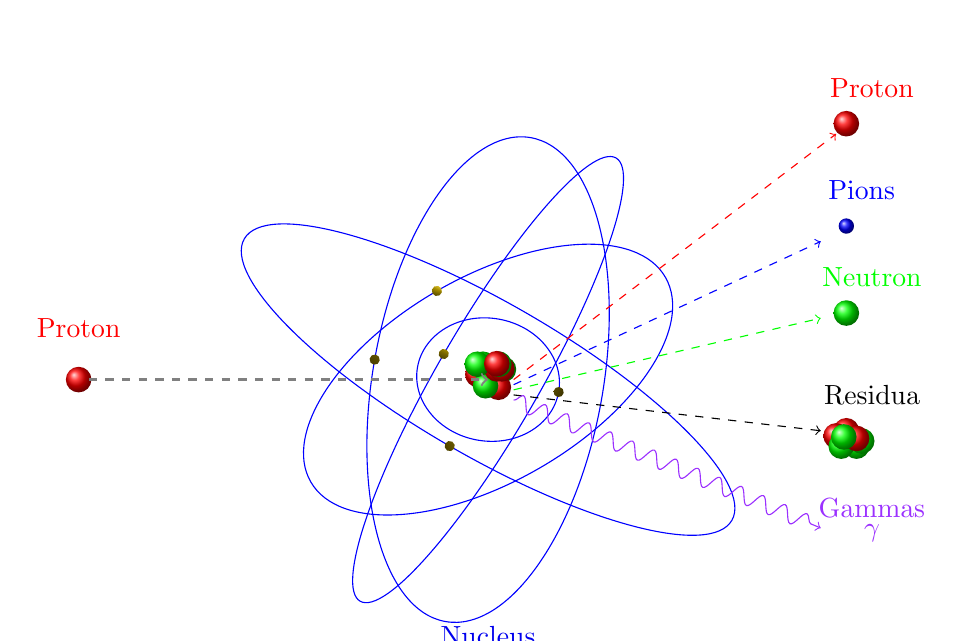
\begin{tikzpicture}[scale=0.65]
		\nucleus
		\proton{-8,0}
		\electron{1.2}{1.4}{260}
		\electron{4}{2}{30}
		\electron{5}{1}{60}
		\electron{5.5}{1.5}{150}
		\electron{4.8}{2.25}{80}
		\proton{7,5}
		\neutron{7,1.3}
		\nucleust
		\pion{7,3}
		\draw[color=Blue2](0,-5) node {Nucleus};
		\draw[blue](7.3,3.7) node {Pions};
		\draw[red](7.5,5.7) node {Proton};
		\draw[red](-8,1) node {Proton};
		\draw[green](7.5,2.0) node {Neutron};
		\draw[color=Purple1](7.5,-2.5) node {Gammas};
		\draw[color=Purple1](7.5,-3) node {$\gamma$};
		\draw (7.5,-0.3) node {Residua};
		\draw [->,color=gray,thick,dashed](-7.8,0) --(0,0); 
		\draw [->,color=red,dashed](0.5,0) --(6.8,4.8);
		\draw [->,color=blue,dashed] (0.5,-0.1) --(6.5,2.7) ;
		\draw [->,color=green,dashed] (0.5,-0.2) -- (6.5,1.2) ;
		\draw [->,,dashed] (0.5,-0.3) -- (6.5,-1.0) ;
		\draw [->,color=Purple1,decorate,decoration={snake,segment length=3mm, amplitude=1mm}] (0.5,-0.4) --(6.5,-2.9) ;
	\end{tikzpicture}
	\caption{Particle emission in the first stage of the spallation reaction}
\end{figure}


For example, the combination of the cascade model of INCL4.6 with the deexcitation model ABLA07
is able \cite{INCLboudard2013new} to describe with the precision of factor 2 the total cross-sections as well as the energy spectra and angular distributions of neutrons, protons and pions for the broad range of the bombarding energies of the light projectile 
(from 50 MeV to 5 GeV). The experimental yields of the remnant nuclei could be reproduced as well. 

However, these models - similarly to all other spallation models - meet a problem of the explanation and quantitative description of the non-equilibrium emission of complex light charged particles (LCP), \emph{i.e.},  $d$, $t$, $^3He$ and $^4He$ as well as of the intermediate mass fragments (IMF), \emph{i.e.}, particles heavier than $^{4}He$ but lighter than products of the fission.



\section{Questions that need to be answered in nuclear spallation research}

After many years of research in this field of experimental and theoretical groups, many fundamental questions are still unanswered. The main of them are:
%the few of them are:
\begin{itemize}
    \item Is the assumption about the two step 
    model justified or the scenario of the reaction is different (e.g., instantaneous formation of a few excited moving sources of particle emission \cite{budzanowski2010comparison}) ? 
	\item What are the mechanisms acting during the initial part of collision? Is the energy/momentum dissipation within the target nucleus realized only by the binary collisions or other mechanisms are present as well ? 
	\item How far it is justified to use the experimental nucleus-nucleus and nucleus-pion cross-sections measured in the vacuum for calculation of collision probability within the nuclear medium ?
	\item What are the mechanisms responsible 
	for the creation of fast composite nuclear particles ?
	\item How far the excited nuclear quantum system can be approximated by the statistical ensemble of point-like particles described by thermodynamics ? 
\end{itemize}	

%	Which of the models of the second stage of the reaction is the best in reproduction of selected observables (total and isotopic cross-sections) -
%	with the assumption that INCL is the best, realistic model of the first stage. On the basis of the literature data.
%	\item The extraction of new experimental DIFFERENTIAL cross-sections of the 
%	protons, pions and deuterons with the aim to check whether INCL is able to reproduce well high energy tail of the spectra (what is necessary to claim that INCL is a good model)
%	\item  To check whether other popular models of the 1st stage are equally good as the INCL model in description of these particles (NOTE: protons are the most abundant charged particles and heavier particles probably may be treated as not important in decision whether the main mechanism is reproduced)
%	\item To check how the properties of the residual nuclei after the 1st stage depend on the applied model 


%	\section{Motivation}
%	It is well known since a long time (cf. \emph{e.g.}, \cite{hyde1971characteristics,korteling1973energy}) that the spallation reactions with emission of LCP and IMF cannot be exclusively described by the emission from the equilibrated remnants of the first stage of the proton-nucleus collisions. Such an emission results in almost isotropic angular distributions whereas it was observed that the spectra of the composite ejectiles are built of two components: the low energy, quasi - isotropic component and the high energy, forward peaked one. Whereas the first component may be attributed to the emission of particles from the equilibrated heavy residuum of the intranuclear cascade the second component is interpreted as the contribution from a non-equilibrium emission of the products. It was found in the papers cited above as well as in many others,\emph{e.g.}\cite{bubak2007non,budzanowski2008competition,budzanowski2009variation,budzanowski2010comparison,fidelus2014sequential,fidelus2017non} that such character of spectra is observed for a broad range of targets (Al, Ni, Ag and Au) as well as for a broad range of the proton beam energies (1.2, 1.9 and 2.5 GeV) and concerns both, LCP and IMF. \par
%	A significant improvement has been achieved in the quantitative description of the non-equilibrium emission of LCP by the INCL4.3 model \cite{boudard2004new} due to the introduction of the surface coalescence of nucleons escaping from the intranuclear cascade stage. This success suggested that the same method might be, perhaps, extended to non-equilibrium emission of IMF. Therefore, further modifications of the INCL were undertaken \cite{boudard2013new}. The resulting version INCL++ of the INCL model considered emission of dynamically created clusters with the mass number A up to 12. However, it turned out that the maximal mass number A of considered IMF has to be in practice limited to values not larger than 8 due to a very long computing time. However, it turned out that very long computing time limited in practice the maximal mass number of considered IMF up to A not larger than 8. Moreover, the spectra predicted by the INCL++/INCL4.6 do not reproduce well the shape of the experimental spectra.  Their slope is always significantly smaller than that observed in the experiment \cite{sharma2016ranking} which leads to the overestimation of the cross-sections at high energies  of emitted IMF with simultaneous underestimation of them at small energies. It is therefore obvious that the invention of another microscopic model is desirable for realistic and efficient description of the non-equilibrium emission of intermediate mass fragments. To achieve such a goal it is necessary to collect %from experimental investigations as many as possible qualitative and quantitative experimental facts on the non-equilibrium processes underlying the IMF, LCP emission.

Some of these fundamental questions are addressed also in this thesis. The general assumption about the two step scenario of spallation process is adopted. 

\section{Organization of thesis}
The review of contemporary theoretical models used for description of the spallation reactions is presented in chapter \ref{chapter:2}. 
The following experimental and theoretical objectives of the present work are discussed in the further chapters of the thesis:

\begin{enumerate}[label=\roman*)]
	\item Studies of the first step of spallation reaction (chapters 3 and 4): 
	the experimental determination of the differential cross-section 
	($d^2\sigma/d\Omega dE$) 
	for emission of Hydrogen isotopes 
	as well as charged pions
	%$\pi^{+}$ and $\pi^{-}$ 
	from collisions of protons 
	with $Nb$ nuclei at $E_p$ = 3.5 GeV (experiment performed in the frame of HADES collaboration) and theoretical description of the obtained data;
%	For this topic 
    \item Second step of the reaction - phenomena governing the deexcitation of the remnant of the first step: 
    the theoretical analysis of the data published in the literature, which contain total isotopic cross-sections for production of nuclei from $Li$ to $Ba$ in $p$+$^{136}Xe$ collision at $E_p$ = 1 GeV. 
% ???    and differential as well as total cross-sections available for p+Ag collisions at Ep=0.48 GeV with production of isotopes of Li, Be, ... Mg nuclei. ???
    Results of this
	analysis were partially published in  \cite{singh2018predictive} and \cite{singh2019odd}. 
	For this subject the chapter 5 is devoted;
	\item Examination of the contribution of the non-equlibrium and equilibruim processes to the total production cross-section for various isotopes and its dependence on the ratio of protons and neutrons in the emitted object (chapter 6). For this aim the data of $p+Ag$ collisions at $E_p$ = 480 MeV published in \cite{Green1984} were utilized;
	\item Theoretical assessment of the experimental observation of variation  
	visible in the total production cross-section for various isotopes of similar mass number A known as Odd-Even Staggering of cross-section (OES). The experimental cross-section are adopted from \cite{Green1984}. This topic is presented in chapter 7.
\end{enumerate}


The thesis is concluded with the summary.

%was to study the mechanisms of pions, proton and nuclear composite particles production in proton-nucleus collisions. The studies were performed partially experimental – utilizing the data of the HADES collaboration and analysing that data to extract the cross-section for p,d,t, and pions, and to some extent theoretical, in the sense that the validation of the existing theoretical models is performed. 
%Two, 
%qualitatively 
%different investigations were undertaken in the present thesis:



 
\chapter{Contemporary theoretical models for spallation reactions}\label{chapter:2}
In this chapter various model describing the mechanism of proton induced spallation reaction will be discussed.As it is described in the Introduction that the spallation reaction is a two step process fist fast stage which occures in few fm/c and second stage is slow stage which occurs in 50 fm/c and excited raminant of is got equilibrated in this stage and the Intermidiate mass fragement (IMF A$>$4) and heavy fragment is emmited in this stage of reaction.
\section{First stage reaction models}
There are various first stage are available which is developed from many decades of the years.I will try to list and describe few of them. 
\subsection{Intranuclear cascade models - INC}
The models which assume, that the interactions of high-energy particles with the nucleus can be represented by free particle-particle collisions inside the nucleus are called intranuclear cascade models. The 1st code of INC has been created by Bertini . In 1963. Later, the conception was used also in other codes, e.g. by Yariv in his ISABEL code. 
In the 80's and 90's, the next versions of INC model was developed by Cugnon et al.(Now known as INCL++ or INCL 4.6 ).
In this thesis only INCL was used for validation of different proton induced reaction. The INCL models are very similar to each other that why I will try to describe the INC models with the example of INCL model.
\subsubsection{Target Nucleus}
The spatial distribution of nucleons inside the target nucleus is prepared according to a Saxon-Woods formula\\
\begin{equation}\label{key}
\rho= \begin{cases} \frac{\rho_{0}}{1+\exp(\frac{R-r_{0}}{a})} &  R<R_{max}\\ 
0 &  R> R_{max} \end{cases} 
\end{equation}
where $R_{max}=r_{int} + R_{0} + a$ and $r_{int}=(\sigma_{NN}^{tot}/\pi)^\frac{1}{2}$
R$_{0}$ and $a$ are taken from electron scattering measurements and parametrized for Al to U as below

\begin{equation}
R_{0}=(2.7545*10^{-4}A_{T}+1.063)A_{T}^{1/3}
\end{equation}
\begin{equation}
a=0.510 + 1.63 *10^{-4}A_{T}
\end{equation}
The initial position and momentum of any target nucleon are generated as follows:is taken at random in a sphere of radius P$_{F}$\\
R(p) is calculated by relation 
\begin{equation}
\left(\frac{P}{P_{F}}\right)^{3}=-\frac{4\pi}{3A_{T}}\int_{0}^{R(p)}\frac{d\rho(r)}{dr}r^{3}dr.
\end{equation}
\subsubsection{Potential}
Isospin and energy-dependent potential well for the
Nucleons
Average potential for pions:  An average isospin dependent Potential well of the Lane type is introduced for pions.
Deflection of charged particles in the Coulomb field: Once an impact parameter is selected for the incident nucleon, the cascade process is initiated with this nucleon located at the intersection of the “external” Coulomb trajectory (corresponding asymptotically to the specific impact parameter) with the “working sphere”.
Nucleons move inside the nucleus along straight trajectories until two of them collide or until one nucleon reaches the nucleus surface, where it can be transmitted or reflected.
Division into participants and spectators.
\subsubsection{Collisions between nucleons}
The collision takes place when the distance between two nucleons is smaller than.
\begin{equation}
d\leq\sqrt{\sigma_{tot}/\pi}
\end{equation}
where $\sigma_{tot}$ is the total nucleon-nucleon cross section
The following possible reactions are considered:
$NN\rightarrow NN, \; NN\rightarrow N\Delta, \; N\Delta\rightarrow N\Delta, \; \Delta\Delta\rightarrow \Delta\Delta, \; \pi N\rightarrow \Delta$
\subsubsection{Pauli Blocking }
The quantum effectsare not totally neglected, i.e. the Pauli blocking is introduced for occupation of the final states which might be populated due to the collision.
The light charged particles (LCP) can be emitted as result of Coalescence .
the stopping time of the cascade is determined self-consistently by the model itself. It parametrized (in fm/c) by:
\begin{equation}
t_{stop}=29.8A_{T}^{0.16}
\end{equation}
\subsubsection{Cluster Emission}
An outgoing nucleon arriving at the surface of the “working sphere,” whether or not it has made collisions earlier, is selected as a possible leading nucleon for cluster emission, provided its energy is larger than the threshold energy, otherwise it is reflected.
Potential clusters are then constructed. The leading nucleon is drawn on its (straight) line of motion back to a radial distance
$D=R_{0}+h$.
\subsection{quantum molecular dynamic (QMD) Models}
\subsection{Jet AA Microscopic Transportation Models (JAM) }
\subsection{Boltzmann-Uehling-Uhlenbeck (BUU) models}
\subsection{Cascade-Exciton model - CEM}
\section{Problem of emission of complex particles}
\subsection{Coalescence}
\section{Models describing the emission from equilibrated remnant}
\subsection{GEM}
\subsection{GEMINI}
\subsection{SMM}
\subsection{ABLA}
\chapter{Mechanisms of proton-nuclear target interaction - studies with HADES spectrometer}\label{chapter:3} %– anisotropic production of pions and H
% isotopes}
\section{p+ Nb @ 3.5 GeV measured in HADES@GSI}
The HADES detection system described in more details in the next chapter permits for registration in broad energy range and clear identification of particles of the interest of this project, namely the π+, π-, p, d, t, 3He, and 4He. Fig. 2 shows the general identification plot of particle species of HADES. Taking advantage of the high resolving power of PID in HADES the main issue will be the proper background estimation and the absolute normalization, taking into account the detection acceptance, efficiency and trigger conditions. For the absolute normalization of measured cross sections, it is planned to utilize the experimental cross section for π- production measured at similar conditions, e.g. in HARP experiment [40-43].  
\section{Description of experiment}
\subsection{RICH}
\subsection{MDC}
\subsection{TOF/TOFino}
\section{Methodology of data analysis}
In order to create the (d2σ/dΩdE) and the (d2σ/dΩ1dΩ2) cross sections the data collected in p+Nb reaction at 3.5 GeV bombarding energy will be used.  The detection system of the HADES experiment is shown in Fig. 3. 
The toroidal magnetic field of HADES system for the momentum measurement together with the precise tracking of 4 layer Mini Drift Chambers (MDC) and particle identification (PID) based on dE/dx information from MDC, TOF and TOFino scintillators will allow to create the double-differential cross sections distributions (d2σ/dΩdE) for LPCs and for pions for emission angles between 18O and 85O. The energy range will cover their almost whole kinematic range. It means that the energy distributions of protons will range from about 50 MeV until about 2.6 GeV (cf. Fig. 2 and 3). It has to be stressed here again that in dedicated experiments oriented for spallation physics [4-9] the particle detection and identification were possible only for energies lower than ~200 MeV cf. Fig. 1 and [3].    
\begin{figure}
  % Requires \usepackage{graphicx}
  \centering\
  \includegraphics{cuts}
  \caption{The scatter plot of dE/dx (MDC) vs. momentum for protons. The cut obtained from 
the asymmetric Gaussian fits is shown. The theoretical calculation of energy loss according to Bethe-Bloch formula is shown as well with the red line.}
  \label{fig:18OGEMINIS2}
\end{figure}
Pion and Light Charged Particle identification in HADES experiment 

For PID in HADES experiment the information from Time of Flight, the dE/dx in MDC detector and dE/dx in TOF and TOFino detectors are used. However, in a few data sets the information on Time of Flight is not available due to hardware constraints. But even in this case, the time of flight can be reconstructed with the use of information from TOF and TOFino detectors (which are the STOP detectors for the time of Flight measurement) and reconstructed track of fast particles like π-.  Such a reference particle has to be detected together with other reaction products what impose the specific the trigger condition, unfavorable measurement of the absolute cross section for single particles. Thus, for creation of a double differential cross section of LCP and pions, the PID of these particles is restricted only to information gained from dE/dx measurements. Nevertheless, the reconstructed Time of Flight of reaction products can be used for rough particle selection with the mass vs. momentum cuts as it is shown in Fig. 5.
In order to obtain the single spectra of LCP and pions the combination of identification methods is done in the following way:
\begin{figure}
  % Requires \usepackage{graphicx}
  \centering\
  \includegraphics{cuts2}
  \caption{The scatter plot of dE/dx(TOFino) vs. momentum (upper panel) and dE/dx(TOF) vs. momentum (lower panel) for proton showing the cuts selecting the protons.}
  \label{fig:18OGEMINIS2}
\end{figure}
1. The mass-momentum distribution is used to define the rough selection cuts for proton, deuteron, triton and pions (cf. Fig. 5).

 
 
Fig. 5. The scatter plot of momentum vs. mass for mesons and LPC registered and identified with the HADES detection system.
 

2. For the selected particles the dE/dx (MDC) vs. momentum plots are done (cf. Example in fig. 6).

3. The projection of dE/dx (MDC) distributions in momentum slices of 25 MeV/c is done. The asymmetric Gaussian fit is applied to each particular distribution in order to define the cuts. The cuts are fixed at (mean 1.5 sigmas) of the fitted functions.

4. Using both the MDC dE/dx (MDC) cut and mass cuts the dE/dx (TOF) and dE/dx (TOFino) vs. momentum are done. The procedure of fitting of the asymmetric Gaussian distribution to the 25 MeV/c momentum slices is applied again.

5. After the final cuts are defined, they are applied to the data set where the mass cut is not used.


\subsection{issues in data analysis}
\subsection{Description of analysis}
\subsection{Establishing of systematic uncertainties}
\chapter{Results of HADES experiment}\label{chapter:4}
\section{Double-differential cross-sections from p +Nb @3.5 GeV}
\section{Comparison with the models}
\section{Interpretation of results}
\section{Interpretation of pi and LCP production}
\section{Conclusion about predictive power of selected models}
  \chapter{Mechanisms of isotropic emission of IMF and heavy target remnants}\label{chapter:5}
  
It was shown in the chapter \ref{chapter:4} that all examined models of the first reaction stage, i.e. INCL++ \cite{INCLMancusi2014}, UrQMD \cite{UrQMDBASS1998,UrQMDBleicher1999} and GiBUU \cite{GiBUUBuss2012}  are almost equivalent in description of the double differential cross-sections for production of light charged particles (LCP). Among these models, the INCL++  has the technical advantage that it can be easily coupled with the de-excitation models such as ABLA \cite{kelic2009abla07}, GEMINI  \cite{CHARITY1988,Charity2010}, GEM  \cite{FURIHATA2000,Furihata2002} and SMM  \cite{SMMBondorf1995}. Moreover, a hypothesis of  coalescence is included for the formation and  emission of lighter composite  particles (A$<$8) during the first stage of reaction. 

In this chapter, presented are the results of the analysis of $^{136}Xe$+$p$ reaction at energy of 
1 GeV/nucleon \cite{napolitani2007measurement}, confronted with the model predictions for the emission of intermediate mass fragments (IMF)  and heavy target residues.
%with the experimental data.

The present analysis was performed in the framework of the two-step microscopic models. The first step of the reaction was simulated by INCL++ (v5.3), which describes the intranuclear cascade of nucleon-nucleon and pion-nucleon collisions. This process leaves an excited heavy remnant in the equilibrium stage. Later, the de-excitation of the equilibrated heavy remnant  is simulated by 4 different theoretical models  \cite{kelic2009abla07,Furihata2002,Charity2010,SMMBondorf1995}. 

The data studied here cover a very wide range of produced elements, from $Li$ (Z = 3) to $Ba$ (Z = 56). This work is a continuation of the recent study \cite{sharma2017ranking}, where the same reactions were analyzed at lower energy (0.5 GeV/nucleon). At that time, the examined data  \cite{giot2013isotopic} included only heavy reaction products, i.e. nuclei from $Nb$ (Z = 41) to $Ba$ (Z = 56). It was found that all the used theoretical models provided reasonable qualitative agreement with the data, although perfect quantitative agreement was not achieved.
%%%


%\section{$^{136}Xe$ + p at 1GeV/A}
%The present analysis was performed in the frame of the
%two-stage microscopic model. The first step of the process
%was described as intranuclear cascade of nucleon-nucleon
%and pion-nucleon collisions leading to the equilibrated, excited
%remnant nucleus. It was realized by the INCL++
%(version 5.3) model \cite{INCLMancusi2014}. The de-excitation of the equilibrated
%heavy products of the first step of the process
%has been calculated in the frame of four different models:
%ABLA07 \cite{kelic2009abla07}, GEM2 \cite{FURIHATA2000,Furihata2002}, GEMINI++ %\cite{CHARITY1988,Charity2010} and
%SMM \cite{SMMBondorf1995}. The physical assumptions of the models as
%well as the details of their realization may be found in
%the references cited above. The most important
%information is already summarized in chapter \ref{chapter:2}.


\section{Analysis of isotopic cross-sections}

The calculations of the isotopic production cross-sections measured by Napolitani et al. \cite{napolitani2007measurement} for the system $^{136}Xe$+$p$ at 1 GeV per nucleon were performed with default values of the parameters of all the models. Therefore it was possible to judge about the predictive power of the applied models. Results of the calculations are presented in figures \ref{Z0314}, \ref{Z1532} and \ref{Z3356} for light ($2 <$ Z $< 15$), intermediate mass ($14 <$ Z $< 33$) and heavy (32 $<$ Z $<$ 57) reaction products, respectively. The qualitative agreement of the theoretical cross-sections with the data will be discussed below for each range of the products separately. 

It is obvious from the inspection of fig. \ref{Z0314} that the GEM2 model underestimates systematically all the data. Furthermore, the theoretical cross-sections decrease much faster with increasing of the atomic number Z than the data. In result the theoretical cross-sections of GEM2 are negligibly small for Z $>$ 9. 

The isotopic cross-sections predicted by other models do not deviate so significantly from the data. Especially, there is not visible such a systematic underestimation of the data as well as its increase with the atomic number. 
All the models produce bell shaped mass distributions of the isotopic cross-sections similar to the distributions of the experimental cross-sections. However, none of the models reproduces exactly the behaviour of the data. 

Absolute values of the cross-sections predicted by ABLA07 for Z $<$ 9 are smaller than those of the data (with exception of the carbon and oxygen isotopes which seem to be well reproduced). The shape of the mass distributions is reasonably well reproduced for given element with exception of fluorine, where the distribution is shifted towards small masses, and aluminium as well as silicon, where the theoretical distributions are too broad. 

The SMM model systematically under-predicts the cross-sections for heaviest isotopes whereas it overestimates the cross-sections for lightest isotopes (with exception of nitrogen where all the models do not work well).

GEMINI++ seems to produce proper width and position of the cross-section distributions, however, it usually under-predicts values of the cross-sections.

\begin{figure}
    \centering
    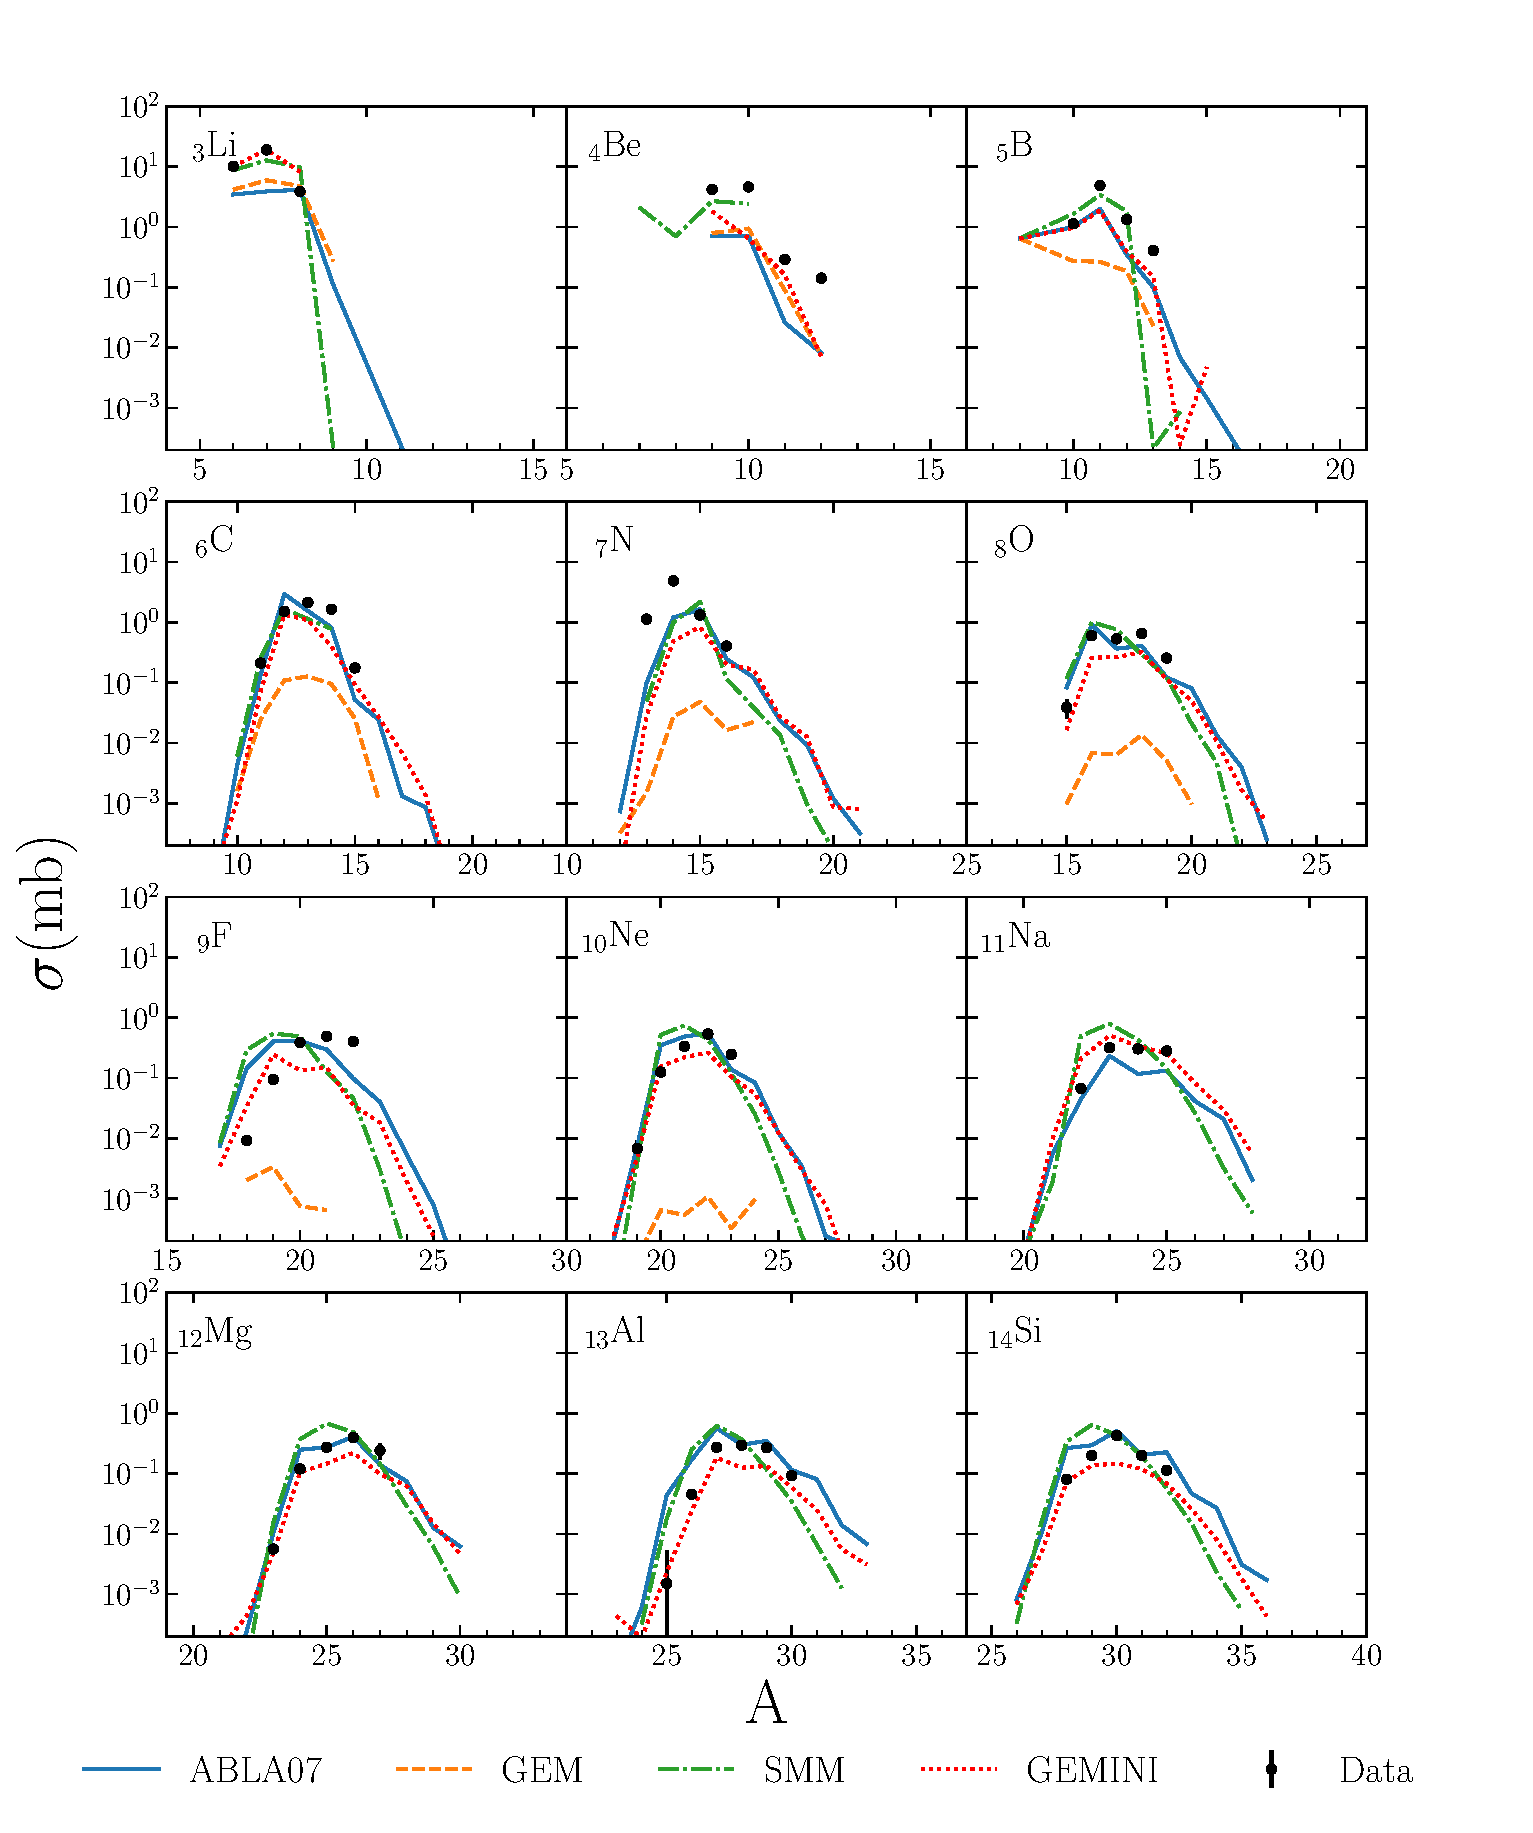
\includegraphics[width=0.9\textwidth]{z0315.eps}
    \caption{Isotopic cross-sections of IMFs with Z = 3–14 from $^{136}Xe$+$p$ collisions at energy T($^{136}Xe$) = 1000 A MeV \cite{napolitani2007measurement} (black dots) together with predictions of the INCL++ (version 5.3) model for the first stage of the reaction coupled to four models of the second stage of reaction: ABLA07 (blue solid line), GEM2 (orange dashed line), GEMINI++ (red dotted line) and SMM (green dashed-dotted line). Note the absence of the theoretical values provided by GEM2 for elements with Z $>$ 10.}
    \label{Z0314}
\end{figure}

The situation is different for elements with 14 $<$ Z $<$ 33. The experimental and theoretical mass distributions of the isotopic cross-sections are presented for these elements in fig. \ref{Z1532}. As can be seen there the GEM2 model does not produce any elements with Z $<$ 30 ($Zn$). Starting from $Zn$ the theoretical cross-sections evaluated with GEM2 appear to be non-negligible but they are more than one order of magnitude smaller than the experimental ones. Thus, the GEM2 cross-sections for the discussed range of elements are completely unrealistic. 

Other models predict the cross-sections which are of the same order of magnitude as the data and, furthermore, the shapes of the mass distributions of the theoretical cross-sections are similar to the shapes of experimental distributions. Nevertheless the systematic deviations of the theoretical cross-sections from the data are observed. 

The mass distributions produced by ABLA07 are too broad in the comparison to the experimental ones. This always leads to the overestimation of the isotopic cross-sections for all isotopes with mass larger than the most populated one and   frequently also for isotopes with the smallest masses. 

The opposite situation is observed for the cross-sections predicted by the SMM model. In this case the cross-sections for isotopes with the smallest mass are systematically overestimated whereas those for the largest masses are systematically underestimated. Thus, in spite of the similarity of the shape of the mass dependence produced by the SMM model and
that observed in the experiment, the absolute values of the cross-sections are systematically overestimated or underestimated by the model. 

Position of the maximum of the mass distribution of the isotopic cross-sections as well as its width is in most cases well reproduced by GEMINI++, however, this model systematically under-predicts the absolute values of the cross-sections. This is most pronounced in the neighbourhood of the maxima of the distributions.

\begin{figure}
    \centering
    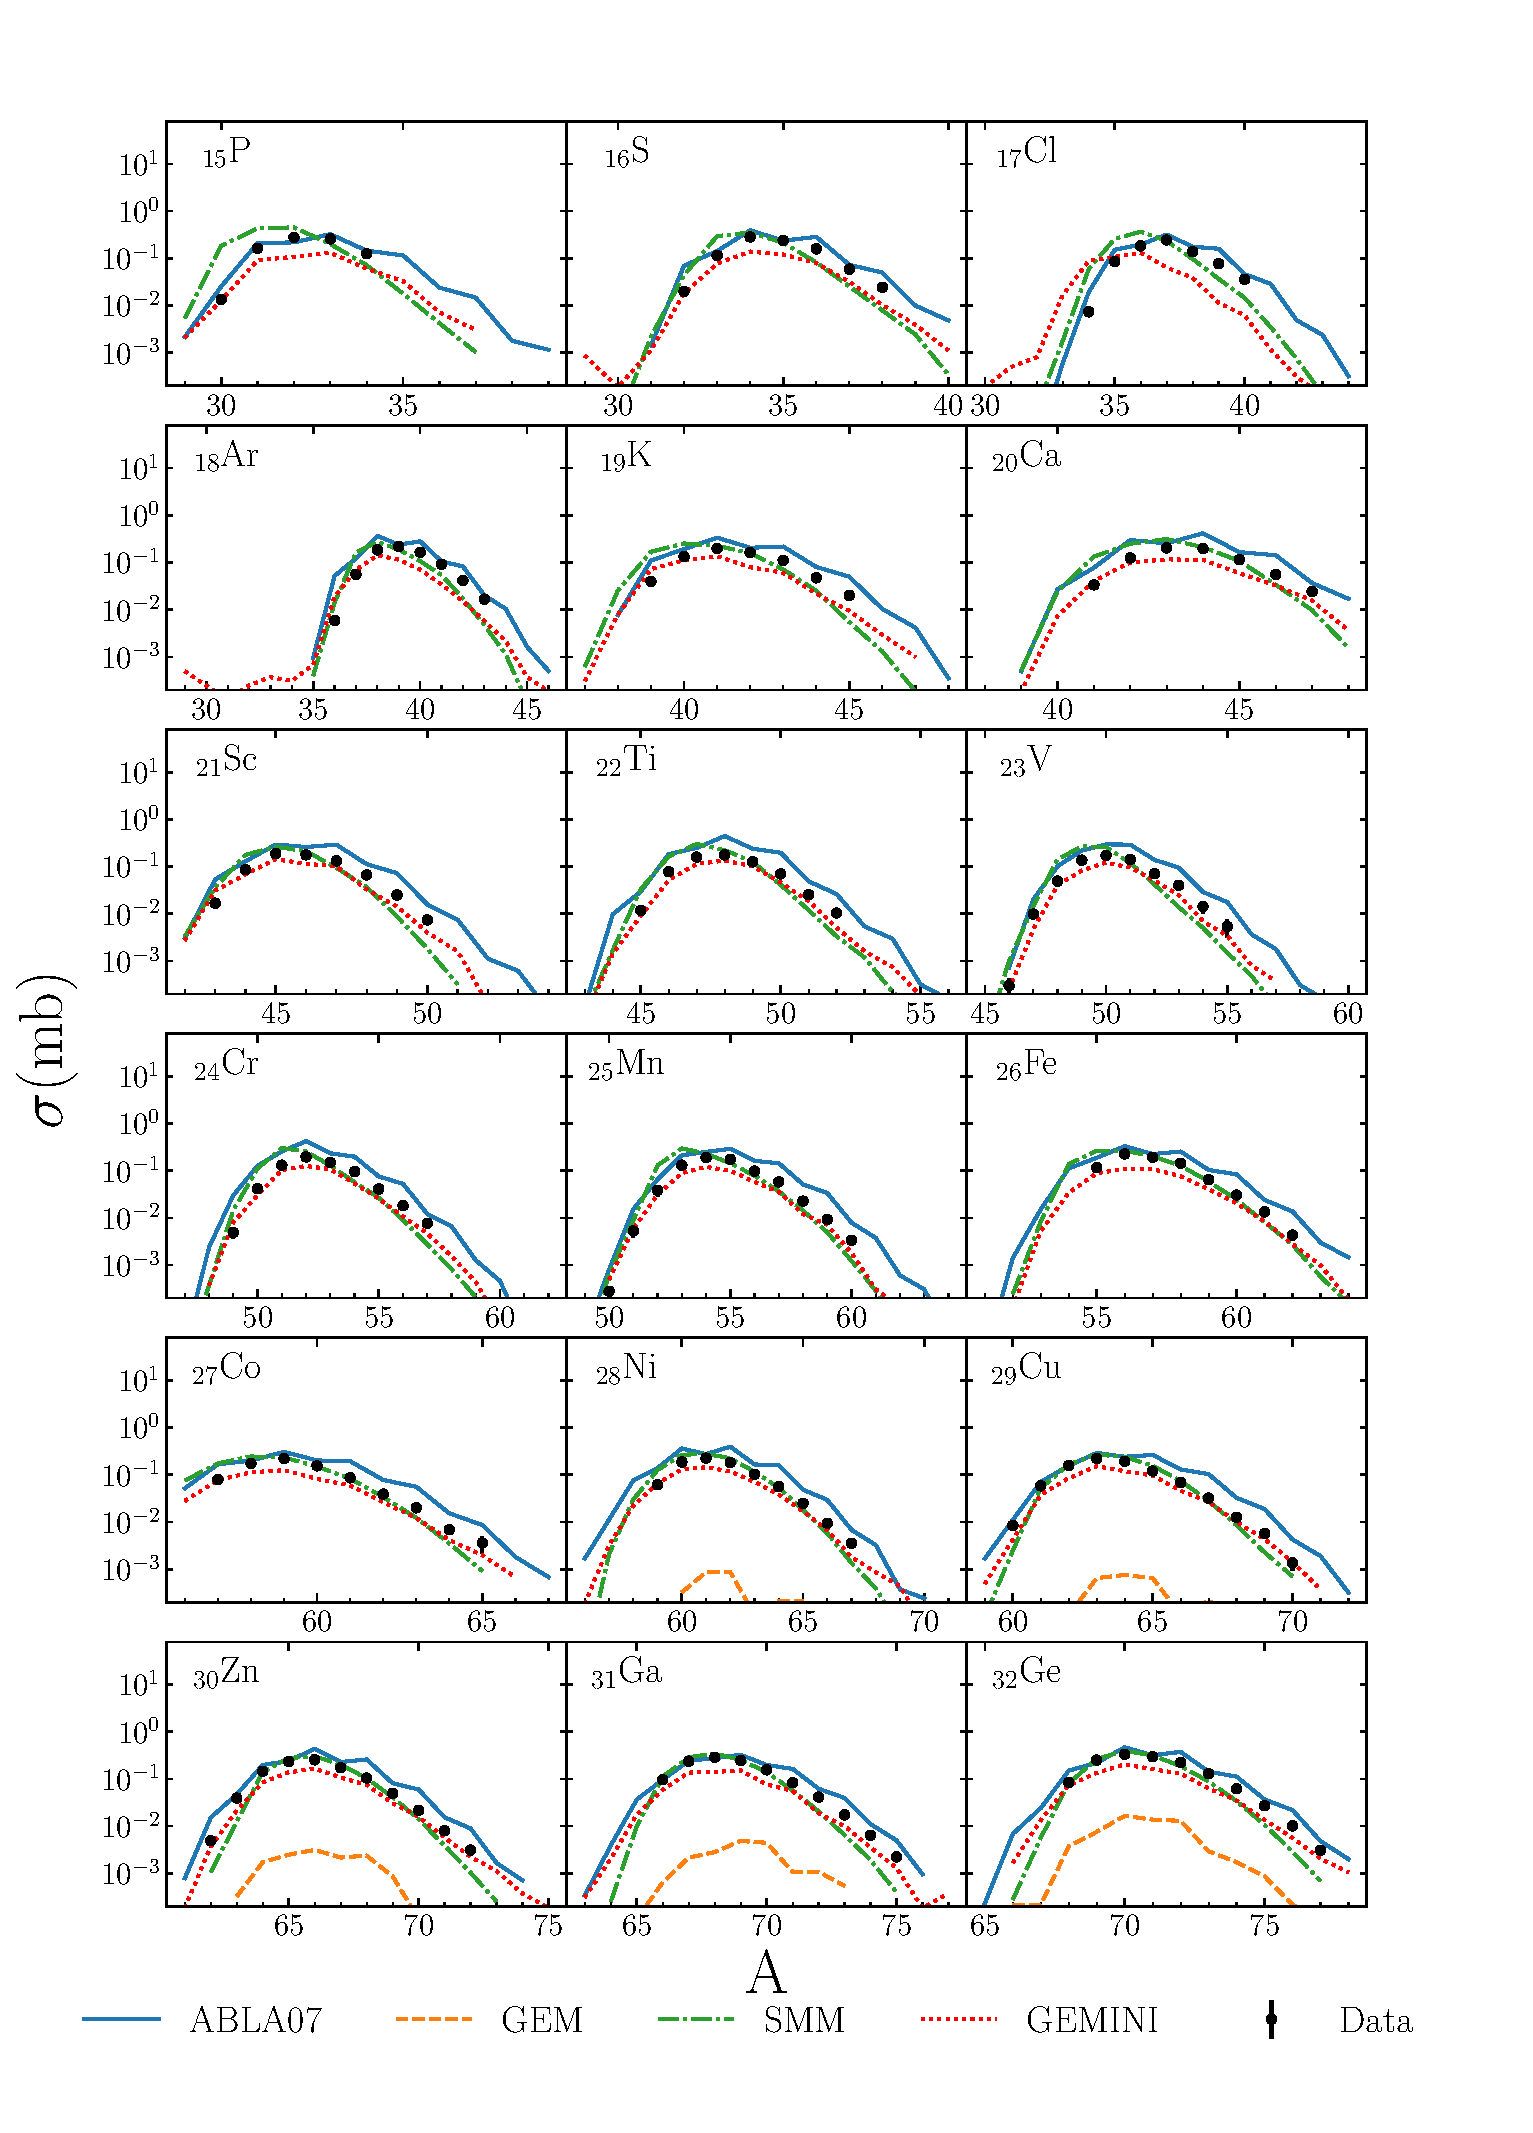
\includegraphics[width=0.93\textwidth]{z1532.eps}
    \caption{The same as in fig. \ref{Z0314}, but for Z = 15–32. Note the absence of the theoretical values provided by GEM2 for elements with Z $<$ 28.}
    \label{Z1532}
\end{figure}
\begin{figure}
    \centering
    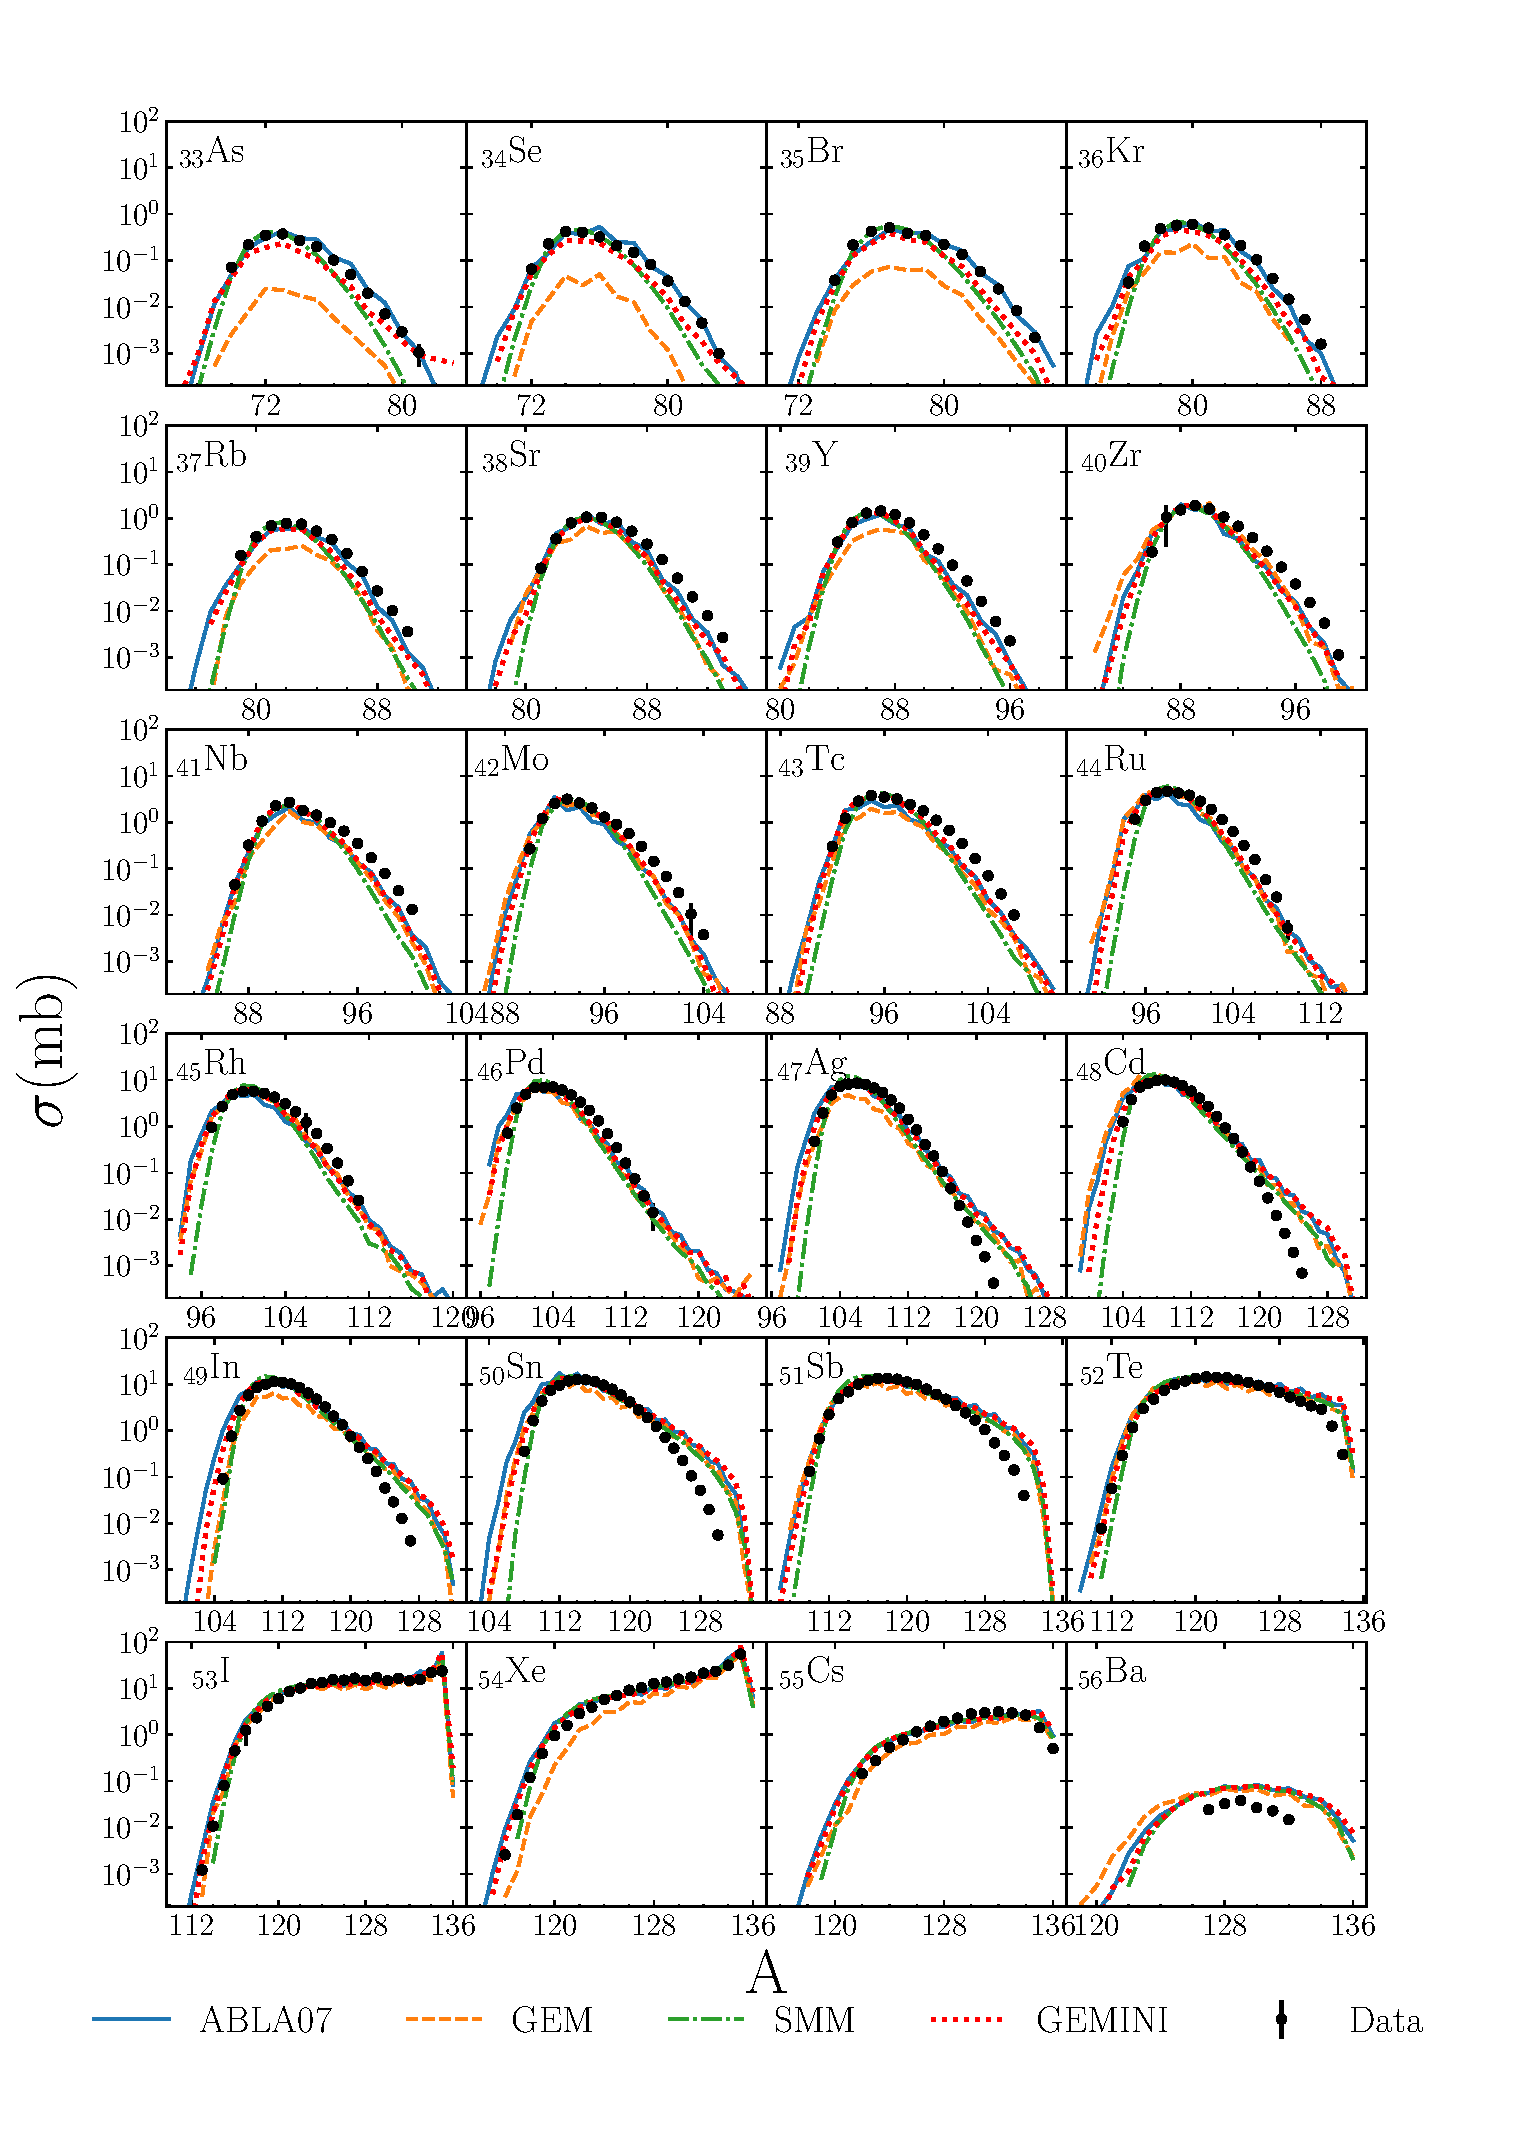
\includegraphics[width=0.95\textwidth]{z3356.eps}
    \caption{The same as in fig. \ref{Z0314}, but for Z = 33–56.}
    \label{Z3356}
\end{figure}

The following qualitative conclusions may be derived from inspection of fig. \ref{Z3356} which presents the isotopic cross-sections measured and calculated for the elements with 32 $<$ Z $<$ 57. The magnitude of the cross-sections predicted by GEM2 model increases with increase of the atomic number of the products. At Z = 33 the model
cross-sections are an order of magnitude smaller than the experimental ones but starting from Z = 40 they start to agree
quite well with the data. The shape of the mass distribution of the isotopic cross-sections predicted by GEM2 for
Z $>$ 40 becomes quite similar to that of the experimental one which is smooth and almost symmetrical up to Z = 47 ($Ac$). 

The other models, i.e., ABLA07, SMM and GEMINI++ reproduce well the shape of the mass dependence
and position of its maximum for all elements starting from Z = 33 ($As$) up to Z = 46 ($Pd$). However, the width of the mass of theoretical and experimental distributions agrees only for ABLA07 and GEMINI++. The SMM model usually
produces too narrow distributions. 

The experimental mass distributions for the range of Z = 47 to Z = 52 of atomic numbers of nuclides (i.e., $Ac$ – $Te$) become asymmetric with the larger values of the cross-sections for the isotopes with large mass number. This behaviour is only partly reproduced by the theoretical models. All of them predict too flat distributions in comparison to the experimental ones. 

As a consequence the values of the experimental cross-sections agree well with the model cross-sections for the lightest isotopes of a given element. They are slightly underestimated for isotopes with average masses and are significantly overestimated (even two orders of magnitude) for the heaviest isotopes. 

The situation changes for reaction products with the largest atomic numbers, i.e., for Z = 53 and Z = 54 ($I$ and $Xe$). In this case the distribution of the isotopic cross-sections monotonically increases with the mass of the  isotopes. All the models reproduce this change of the character of the distributions as well as the magnitude of the cross-sections. The GEM2 model seems to be the poorest in reproduction of $Xe$ (Z = 54) isotopic cross-sections, however it describes well the isotopic cross-sections for $I$ (Z = 53) and $Cs$ (Z = 55). The experimental distribution of the isotopic cross-sections for the element with the largest Z (Z = 56), i.e., for $Ba$, is systematically overestimated by all theoretical models.


\section{Predictive power of the de-excitation models and range of their usage}

The detailed discussion of the agreement between model and experimental isotopic cross-sections presented above does not permit to make a simple, general overview of the quality of description of the data by all examined models. To allow for such an overview the following procedure was applied. 

All isotopes for which the production cross-sections were determined in the experiment \cite{napolitani2007measurement} are presented as empty circles in the two dimensional plot (Z-N) in fig. \ref{ZAfactor}. The isotopes for which the model cross-sections do not deviate more than 10$\%$ from the data are shown as full circles. 

This specific value of the relative deviation was chosen somewhat arbitrary taking into  consideration that the typical relative errors estimated for the most abundant isotopes in the experiment \cite{napolitani2007measurement} are equal to 5$\%$–6$\%$ and do not overcome 20$\%$. 

It may be concluded after inspection of fig. \ref{ZAfactor} that such a representation allows to observe 
characteristic behaviour of the quality of data  reproduction by different models:

\begin{enumerate}[label=\roman*)]
    \item  The number of well described data is rather small. About 12$\%$ of the experimental cross-sections are well reproduced by ABLA07, SMM and GEMINI++ whereas only about 4$\%$ in the case of the GEM2 model.
    
    \item The cross-sections for products with large atomic number Z are more frequently reproduced by the models
    than those for products with small Z. This is especially pronounced in the case of GEM2 where the only reproduced
    experimental cross-sections are those for large Z.

    \item In the case of GEMINI++ several neighbouring isotopes of the same element with the large Z are very well
    reproduced. This is however not the case for other models. It indicates that for these elements GEMINI++ well reproduces
    the shape of the N-dependence of the experimental cross-sections (at least for the largest N values, cf. fig. \ref{Z3356}).
    A quite different situation is present for SMM where two or three lines of well reproduced (Z-N) cross-sections are
    visible. It is caused by the fact that the shape of the mass dependence of isotopic cross-sections predicted by SMM
    is different than the experimental shape. Due to this fact the experimental and theoretical N distributions for given Z
    are crossing at two or three N values (cf. fig. \ref{Z3356}). 

    \item The data for elements with 30 $<$ Z $<$ 40 are not reproduced by GEMINI++ and GEM2 but the ABLA07
    and SMM predictions agree well with the data.

    \item  The data for elements with 20 $<$ Z $<$ 30 are not described by GEM2 and ABLA07 whereas SMM and GEMINI++
    work well for this range of the atomic number.

    \item Isotopic cross-sections for elements with 10 $<$ Z $<$ 20 are not reproduced by GEM2 but some of them are well described by other models.

\end{enumerate}
It is worth emphasizing that different models describe
well different isotopes for this range of atomic number:
GEMINI++ is good for the smallest N-values whereas
ABLA07 and SMM for average N. ABLA07 and 
SMM reproduce well the maximal isotopic  cross-sections 
for given Z. This specific behaviour is caused by the shift 
of the mass distributions produced by ABLA07 and SMM 
towards small N values with respect to the experimental
distributions - cf. fig. \ref{Z0314}.
\begin{figure}
    \centering
    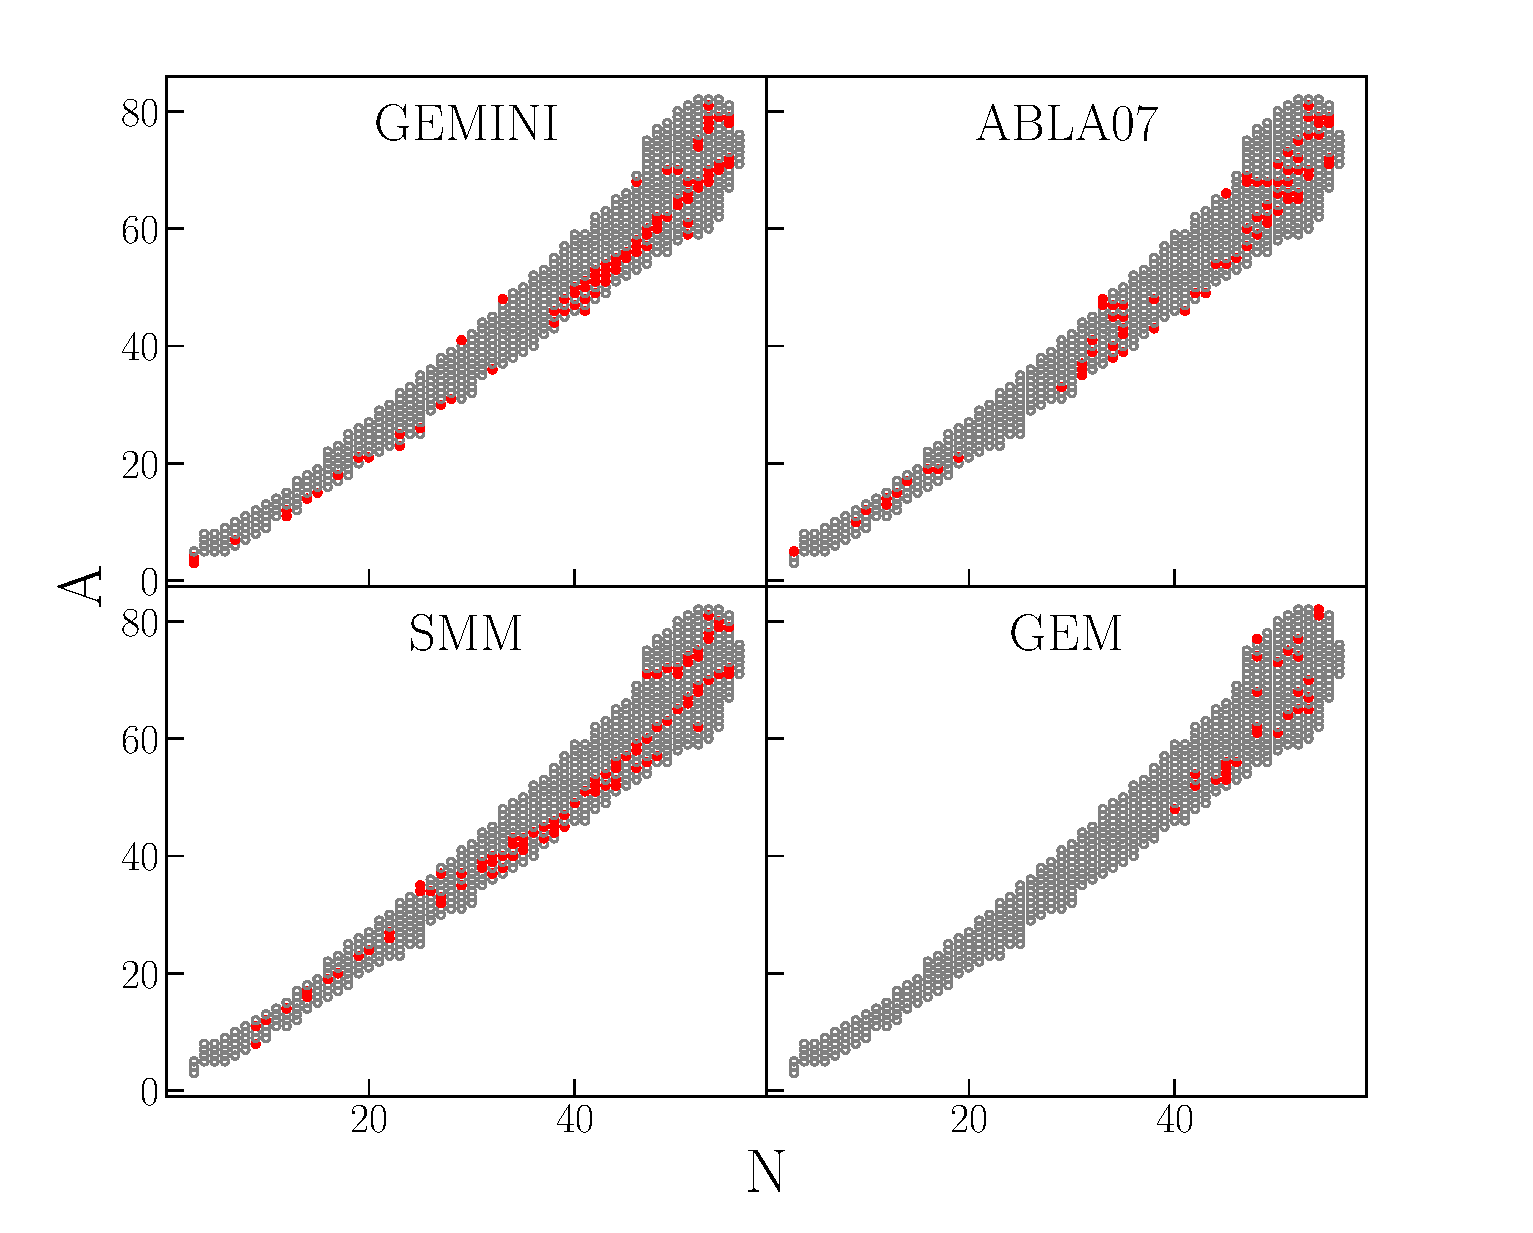
\includegraphics[width=0.85\textwidth]{ZA_Afactorall.eps}
    \caption{The values (Z,N) of experimentally obtained isotopic cross-section in  \cite{napolitani2007measurement} for $^{136}Xe$+$p$ reaction at energy 1 GeV/nucleon (empty circles). The values (Z,N) at which the relative deviation between theoretical ($\sigma^{th}$) and experimental ($\sigma^{exp}$) cross-sections calculated as $2\cdot\left| \sigma^{th}- \sigma^{exp} \right|/(\sigma^{th} + \sigma^{exp})$ is smaller than 10$\%$ are marked with full red circles. The left upper panel contains results of GEMINI++, the right upper panel contains results of ABLA07, the left lower panel contains results of SMM and the right lower panel contains those of GEM2.}
    \label{ZAfactor}
\end{figure}

Another representation of the quality of the model predictions for the isotopic 
cross-sections is application of the $A$-factor (defined in chapter \ref{chapter:4}, formula \ref{A_factor_1}). As it was discussed there  values of the $A$-factor for well predicted 
cross-sections are close to zero. 

The $A$-factor values calculated in this investigation for all the data and for  corresponding combinations of models are presented in fig. \ref{Afactorall}. 

As can be seen in this figure the $A$-factor evaluated
for the GEM2 model cross-sections differs strongly from all others cases. It has values close or equal to one for all
elements with Z between 9 and 30. This is due to the
fact that GEM2 does not produce ejectiles 
in this range of the atomic number Z. 

Other models, which better
reproduce the data provide smaller values of $A$-factor varying between 0.1 and 0.6. 

The following interesting conclusions may be derived from inspection of fig. \ref{Afactorall}:

\begin{figure}
    \centering
    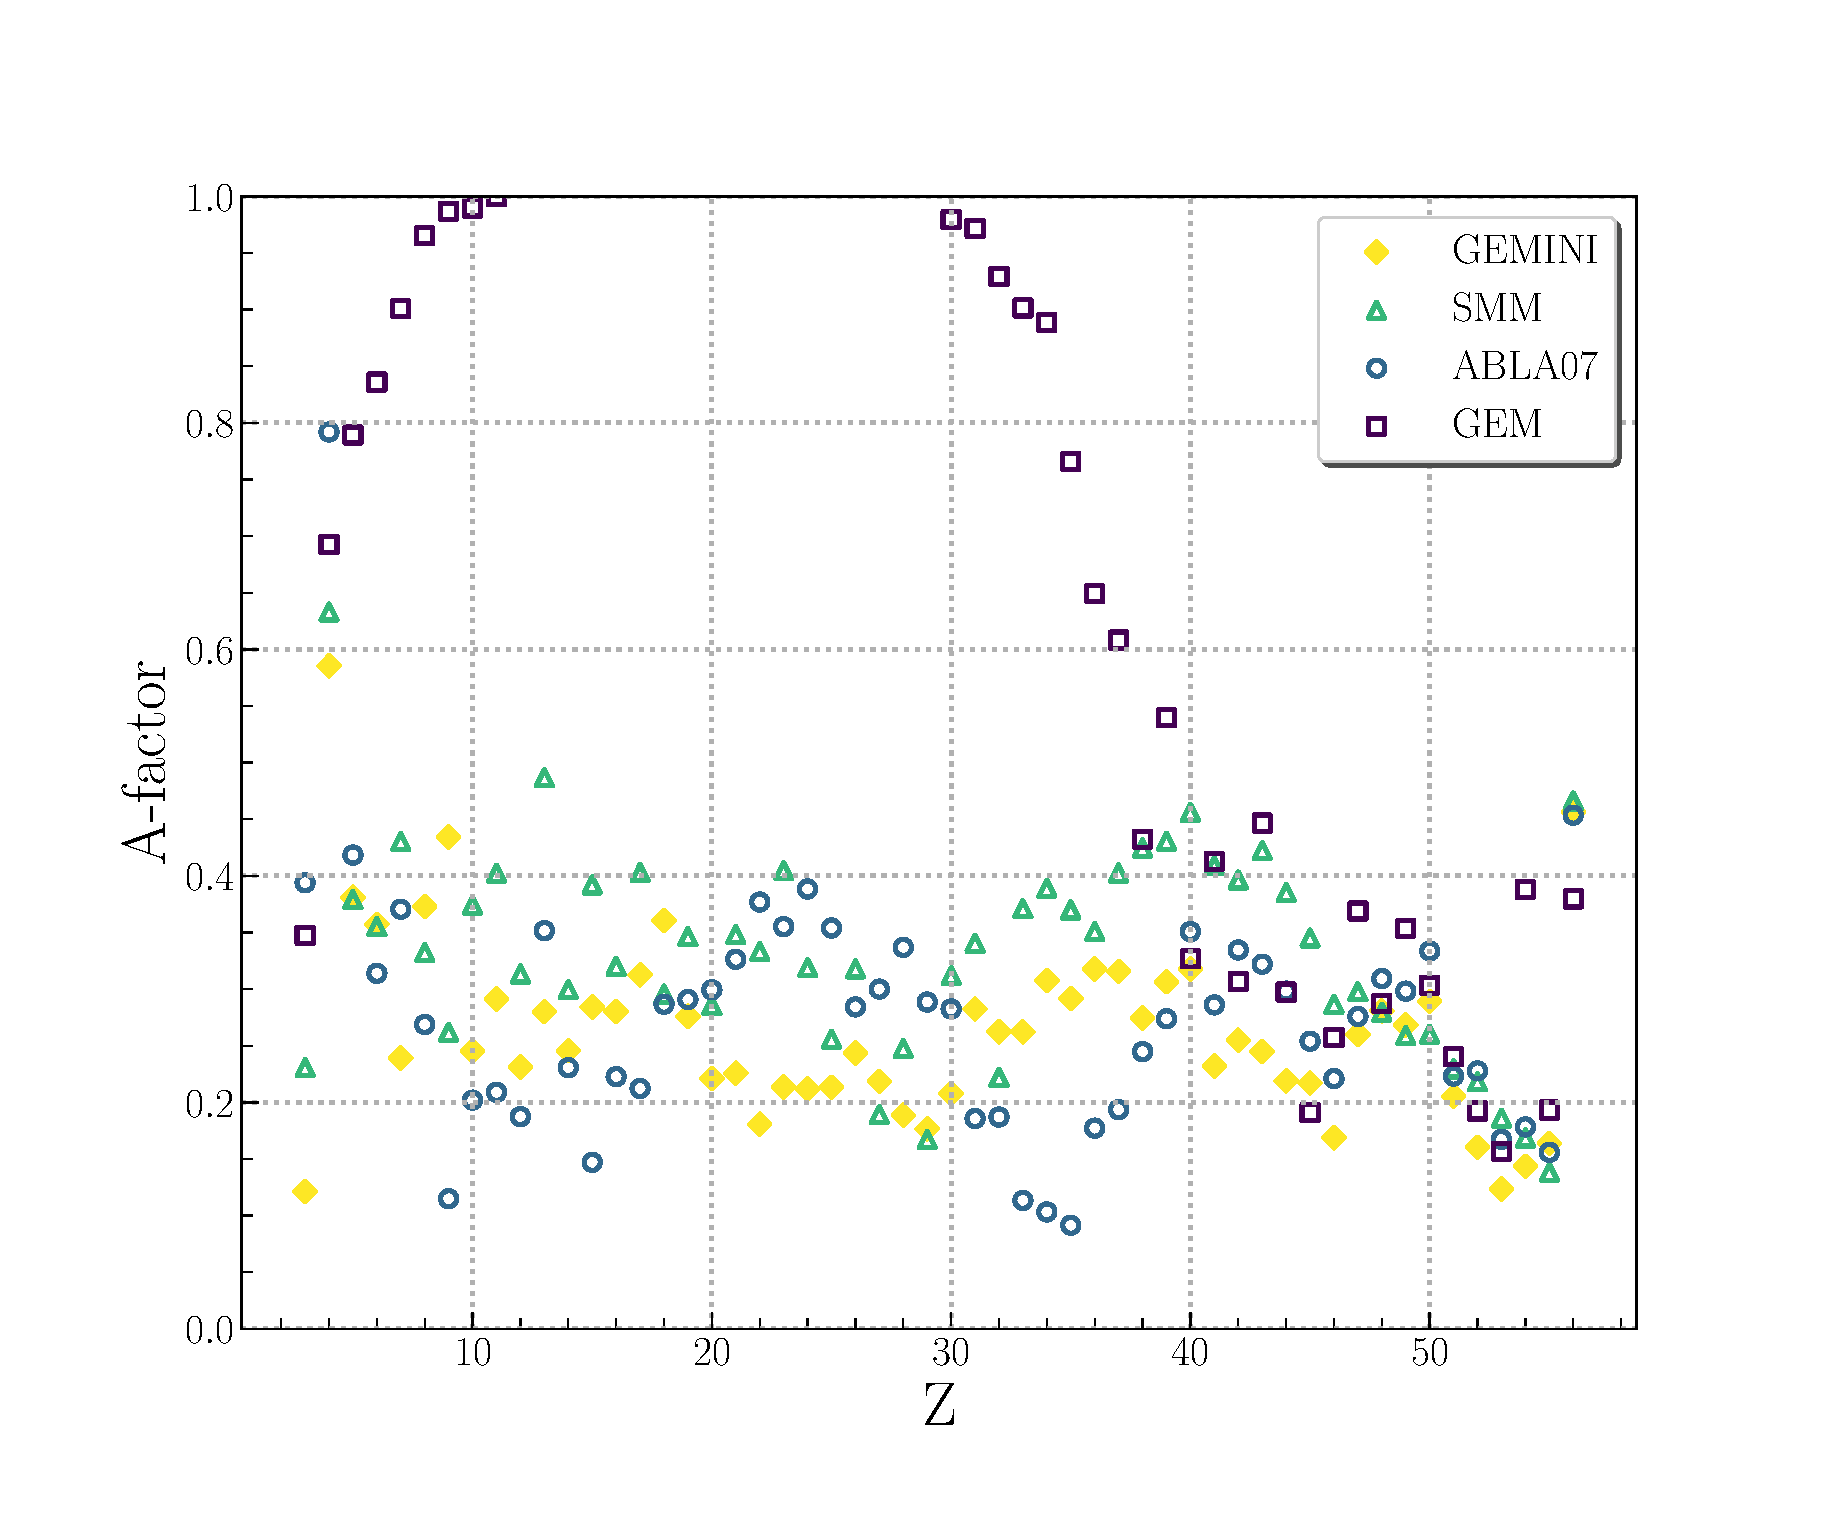
\includegraphics[width=0.9\textwidth]{Afactorall.eps}
    \caption{Values of the $A$-factor evaluated according to equation \ref{A_factor_2}. 
    Blue, open circles represent results obtained for ABLA07, violet open squares correspond to GEM2, green open triangles to SMM whereas yellow solid diamond show values calculated for GEMINI++ results.}
    \label{Afactorall}
\end{figure}
\begin{itemize}
    \item[i)]  The data with 47 $<$ Z $<$ 55 are equally well reproduced
by all the models. This is the range of elements
which are mainly produced by the evaporation of nucleons
from the excited remnant of the intranuclear
cascade.
\item[ii)] For products with 40 $<$ Z $<$ 47 the GEMINI++ model is the best
in reproducing the data. The SMM is the worst 
one in this respect. Results of ABLA07 are randomly better or poorer than those of GEM2.
\item[iii)] The ABLA07 gives distinctly the best description of
the products with 30 $<$ Z $<$ 40. GEMINI++, SMM
and GEM2 lead to the poorer reproduction of the data
with the quality decreasing in the indicated sequence.
\item[iv)] The situation changes for products with 18 $<$ Z $<$ 30
where the GEMINI++ offers the best description of
the data. ABLA07 and SMM compete to provide second
the best reproduction of the experimental cross
sections. The GEM2, which does not produce ejectiles
for this range of atomic number is completely not applicable.
\item[v)] The lowest range of atomic numbers, i.e., Z $<$ 19
seems to be the best described by ABLA07 whereas
GEMINI++ and SMM give comparable, slightly
poorer description.
\end{itemize}
     \begin{longtable}[c]{| c || c |c|c|c|}
     \caption{Ranks of theoretical predictions  of examined in this study models for isotopic distributions
of residua from $Xe$+$p$ collisions at 1 GeV/nucleon \cite{napolitani2007measurement}
according to values of the $A$-factor. For explanation see text. \label{ranktable_long}}\\
     \hline
    \multirow{2}{4em}{Ejectile} &\multicolumn{4}{|c|}{The ranks of the models}\\
    \cline{2-5}
    & ABLA07& GEM2& GEMINI++& SMM\\
    \hline
    \hline
    \endfirsthead
    \hline
 \multicolumn{5}{|c|}{Continuation of Table \ref{ranktable_long}}\\
 \hline
 Ejectile & ABLA07& GEM2& GEMINI++& SMM\\
 \hline
 \hline
    \endhead
\hline
 \endfoot

 \hline
 \hline
Sum of ranks & 116& 195& 91& 138\\
 \hline
  \hline
 Average rank: & 2& 4& 1& 3\\
 \hline
 \endlastfoot
$_{3}$Li & 4 & 3 & 1 & 2 \\
$_{4}$Be & 4 & 3 & 1 & 2 \\
$_{5}$B & 3 & 4 & 2 & 1 \\
$_{6}$C & 1 & 4 & 2 & 3 \\
$_{7}$N & 2 & 4 & 1 & 3 \\
$_{8}$O & 1 & 4 & 3 & 2 \\
$_{9}$F & 1 & 4 & 3 & 2 \\
$_{10}$Ne & 1 & 4 & 2 & 3 \\
$_{11}$Na & 1 & 4 & 2 & 3 \\
$_{12}$Mg & 1 & 4 & 2 & 3 \\
$_{13}$Al & 2 & 4 & 1 & 3 \\
$_{14}$Si & 1 & 4 & 2 & 3 \\
$_{15}$P & 1 & 4 & 2 & 3 \\
$_{16}$S & 1 & 4 & 2 & 3 \\
$_{17}$Cl & 1 & 4 & 2 & 3 \\
$_{18}$Ar & 1 & 4 & 3 & 2 \\
$_{19}$K & 2 & 4 & 1 & 3 \\
$_{20}$Ca & 3 & 4 & 1 & 2 \\
$_{21}$Sc & 3 & 4 & 1 & 2 \\
$_{22}$Ti & 3 & 4 & 1 & 2 \\
$_{23}$V & 2 & 4 & 1 & 3 \\
$_{24}$Cr & 3 & 4 & 1 & 2 \\
$_{25}$Mn & 3 & 4 & 1 & 2 \\
$_{26}$Fe & 3 & 4 & 2 & 1 \\
$_{27}$Co & 3 & 4 & 2 & 1 \\
$_{28}$Ni & 3 & 4 & 1 & 2 \\
$_{29}$Cu & 3 & 4 & 2 & 1 \\
$_{30}$Zn & 3 & 4 & 1 & 2 \\
$_{31}$Ga & 1 & 4 & 3 & 2 \\
$_{32}$Ge & 1 & 4 & 3 & 2 \\
$_{33}$As & 1 & 4 & 2 & 3 \\
$_{34}$Se & 1 & 4 & 2 & 3 \\
$_{35}$Br & 1 & 4 & 2 & 3 \\
$_{36}$Kr & 1 & 4 & 2 & 3 \\
$_{37}$Rb & 1 & 4 & 2 & 3 \\
$_{38}$Sr & 1 & 4 & 2 & 3 \\
$_{39}$Y & 1 & 4 & 2 & 3 \\
$_{40}$Zr & 3 & 2 & 1 & 4 \\
$_{41}$Nb & 2 & 3 & 1 & 4 \\
$_{42}$Mo & 2 & 3 & 1 & 4 \\
$_{43}$Tc & 2 & 4 & 1 & 3 \\
$_{44}$Ru & 3 & 2 & 1 & 4 \\
$_{45}$Rh & 3 & 1 & 2 & 3 \\
$_{46}$Pd & 3 & 2 & 1 & 3 \\
$_{47}$Ag & 1 & 4 & 1 & 3 \\
$_{48}$Cd & 3 & 2 & 1 & 3 \\
$_{49}$In & 3 & 4 & 1 & 1 \\
$_{50}$Sn & 3 & 3 & 2 & 1 \\
$_{51}$Sb & 2 & 4 & 2 & 2 \\
$_{52}$Te & 3 & 3 & 3 & 1 \\
$_{53}$I & 3 & 1 & 3 & 2 \\
$_{54}$Xe & 3 & 4 & 2 & 1 \\
$_{55}$Cs & 2 & 4 & 2 & 1 \\
$_{56}$Ba & 2 & 4 & 2 & 2 \\
\end{longtable}
To summarize this analysis quantitatively, the ranks 
of the models based on values of the $A$-factor were collected
in table \ref{ranktable_long}.
%for all elements produced in the studied here 
%reaction. 
A smaller rank of the model for a given element
means that the model leads to a smaller value of  $A$-factor, thus provides the better description of the data.

If two models give practically the same value of the $A$-factor
then the arithmetic average of their ranks is quoted
in table \ref{ranktable_long} for both models.

The sum of the ranks for a given theoretical 
model for all observed elements can be treated
as a quantitative measure of the quality of its  data description.
%of all the data by the model under consideration.

As can be learn from table \ref{ranktable_long} the quality of the overall 
description of the examined data is the best for GEMINI++ (sum of the ranks is equal to 91). 
The second place in the description of experimental data
is granted to ABLA07 (sum equal to 116). The
third in this respect is SMM (sum equal to 138) and the poorest description of the data is obtained with the use of GEM2 model (sum of ranks equal to 195).

\section{Conclusions about examined second step reaction models}

A very rich set of production cross-sections (over 600) 
%cross-sections) 
measured by Napolitani et al. \cite{napolitani2007measurement} with
isotopic identification of the products for $^{136}Xe$+$p$ collisions
at 1 GeV per nucleon was compared with predictions 
of a two-step reaction scenario simulated with  microscopic theoretical models. 

The first stage of
the reaction was analyzed in the frame of the INCL++
model \cite{INCLboudard2013new}. It treats the proton-nucleus collision as a
sequence of nucleon-nucleon and nucleon-pion collisions
leaving the equilibrated, excited remnant nucleus. 

The description of the second
stage of the reaction was tested with the use 
of four different models: ABLA07  \cite{kelic2009abla07}, GEM2  \cite{FURIHATA2000,Furihata2002}, GEMINI++ \cite{CHARITY1988,Charity2010} 
and SMM \cite{SMMBondorf1995}. They assume different scenarios of the
de-excitation process of the intranuclear 
cascade remnant.

All calculations were performed using the default values
of the applied theoretical models with the aim to study
the predictive power of the models in respect to the determination
of isotopic cross-sections.

It was found that ABLA07, SMM and GEMINI++ reproduce
the main properties of the Z and A dependence of the cross-sections for reaction products which cover very
broad range of elements (from $_{3}Li$ to $_{56}Ba$) whereas the
GEM2 gives comparably good predictions only for lithium
and for the elements with large atomic number (Z $>$ 40).

This is illustrated by figs. \ref{Z0314}, \ref{Z1532} and \ref{Z3356}, which present the data and
the theoretical cross-sections for separate ranges of atomic
number Z of the products. Inspection of these figures allows
to estimate qualitatively the agreement between the 
data and the model predictions.

A very good quantitative reproduction of the experimental
isotopic cross-sections, i.e., such which results in
the relative deviation between the data and the model
cross-sections smaller than 10\%, was achieved only for a
small part of all the cross-sections as it is shown in fig. \ref{ZAfactor}.

The models ABLA07, SMM and GEMINI++ offer such a
perfect reproduction of data for approximately 12\% of the
products whereas GEM2 only for approximately 4\%. This
suggests that the models under consideration cannot be
approved if the main criterion would be the  perfectness of the cross-sections prediction 
for isotopically resolved reaction products.

Better but also not perfect prediction of the cross-sections
was found when the average agreement over isotopes
of given element is considered. Such a quantitative comparison
of the model and experimental cross-sections was
achieved by the application of the $A$-factor  which was described in chapter \ref{chapter:4}. 

%a reference \cite{sharma2017ranking}  
%dealing with the reactions in the same nuclear system,
%i.e., $^{136}Xe$ + p but at twice smaller energy (500MeV per nucleon). 

The Z-dependence of the $A$-factor presented in
fig. \ref{Afactorall} shows that the production cross-sections of elements
with largest atomic numbers are equally well reproduced
by all applied models. The situation changes for
smaller atomic numbers. Then the different models assure the
best description for different ranges of the atomic number
of products. 

The ranking of models based on achieved values
of the $A$-factor was made (cf. table \ref{ranktable_long}) which clearly
shows that the averaged over isotopes and elements agreement
between the data and experimental cross-sections is
the best for GEMINI++. 
The ABLA07 and SMM produced
poorer average agreement and the GEM2 is the
worst.

These conclusions agree with result obtained in the work \cite{sharma2017ranking} in which the analysis of the data measured 
at lower energy, i.e., 500 MeV per nucleon for the
same nuclear system were investigated. 
But then only elements with Z $>$ 40 were studied. 

%The data were reproduced
%in the best way by GEMINI++, however the SMM
%model gave better description than ABLA07 whereas
%GEM2 also achieved the last position. The conclusion that
%the values of the $A$-factor are too big to claim that the
%studied models may be approved remains true also after the present analysis.

\chapter{The yields of non-equilibrium and equilibrium processes in spallation reactions (IMF)}\label{chapter:6}
 To estimate experimentally the relative rate of non-equilibrium
processes one has to know both, the total production cross section
of given IMF and the cross section for its non-equilibrium emission.
The total production cross section may be in principle obtained by a
straightforward integration over energy and scattering angle of the
experimental differential cross sections $d\sigma/d\Omega dE$,
however the production cross section of given IMF due to a
non-equilibrium process cannot be extracted from the experiment
without additional model assumptions.  The most promising method for
this purpose seems to be substraction of the \emph{equilibrium}
emission cross section of given IMF  from its total production cross
section. Such a method should give value of the non-equilibrium
production cross section as reliable as that of the equilibrium
emission processes.  %Since the models which describe  emission of
%fragments from excited, equilibrated nuclei have been developed and
%improved since a very long time it is reasonable to expect that
%their predictive power is much better than that of other reaction
%mechanisms.
\section{IMF production cross sections in p + Ag reaction at 480 MeV}


It was demonstrated in the recent publications concerning predictive
power of various reaction models used for the description of
isotopic production cross sections in p+$^{136}$Xe collisions at 1
GeV/nucleon \cite{singh2018predictive} and at 0.5 GeV/nucleon \cite{sharma2017ranking}
as well as for the analysis of differential cross sections of
spallation reactions in p+Ag collisions at 0.48 GeV/nucleon
\cite{sharma2016ranking} that the description of data by GEMINI model\cite{CHARITY1988,Charity2010}[ref AIEEE] coupled to INCL4.6
\cite{boudard2013new} is superior in respect to those obtained with
three other, popular models of the second stage of the reaction,
namely ABLA07 \cite{ABLA07}, SMM \cite{Bondorf95A} and GEM2
\cite{Furihata00A,Furihata02A}. Moreover, it was found that among
the above listed models only GEMINI does not produce cross sections
which exceed magnitude of the experimental data leaving a room for
another reaction mechanism contributing incoherently to the
reactions studied \cite{Sharma16A}.




The following procedure has been used for the estimation of the
equilibrium processes contribution to the production of the
intermediate mass fragments. It was assumed that the collision of
proton impinging on to the silver target proceeds as the two step
process. The INCL++ model (version 5.3) \cite{Mancusi14A} of the
intranuclear cascade has been used for description of the first,
fast stage of the collisions.
%
%The first, fast stage of the reaction consists in intranuclear
%cascade of nucleon-nucleon and nucleon-pion collisions which at the
%end leaves the excited, residual nucleus in the thermodynamical
%equilibrium. Such a compound nucleus decays further by emission of
%nucleons, light charged particles (LCP) and intermediate mass
%fragments (IMF) eventually (for the heaviest atomic nuclei) it may
%be a subject of nuclear fission.
%
%In the present study the INCL++ model (version 5.3)
%\cite{Mancusi14A} of the intranuclear cascade has been used.
%
A possibility of the emission of complex light charged particles in
this stage of the process has been taken into account to assure
achieving a realistic mass, charge and excitation energy
distribution of the residual compound nuclei. However, the
coalescence of the nucleons escaping from the intranuclear cascade
with creation of intermediate mass fragments was not allowed because
of two reasons: (i) the INCL++ enables one to perform efficiently
such calculations only for the lightest IMF \cite{Boudard13A} and,
(ii) it was found in the earlier study of these reactions
\cite{Sharma16A} that high energy spectra of IMF are significantly
overestimated by this model.  It is important to emphasize that the
above decision does not modify significantly the mass, charge and
energy distribution of the excited nuclei - the remnants of the
cascade since the cross sections for production of IMF are orders of
magnitude smaller than those for nucleons and complex LCP. The
second stage of the process, i.e., emission of particles from the
excited compound nuclei - residuals of the fast stage of the
reactions was described by GEMINI++ model \cite{GEMINI++}.  The
results of the above calculations were treated as a realistic
estimation for the total as well as for differential cross sections
of equilibrated emission of IMF.

To obtain the total production cross section, the GEMINI++ double
differential cross sections $d^2\sigma/dEd\Omega$ were supplied by
incoherently added isotropic emission from highly excited Maxwellian
source (or two sources) moving along the beam direction. The
parameters of the source, i.e., its velocity $\beta$, apparent
temperature T, the contribution to the total cross section $\sigma$
and the parameters responsible for the Coulomb barrier hindering the
emission of ejectiles from the source were fitted to reproduce
simultaneously the spectra of given ejectile at all scattering
angles. Details of the moving source model as well as the
interpretation of its parameters  can be found in the Appendix of
Ref. \cite{Bubak07A}.

Very good reproduction of most of the data was achieved using one
moving source contribution. %to represent non-equilibrium part of the
%cross sections.
This is illustrated by Fig. \ref{fig:18OGEMINIS2} in which
experimental (dots) and model (lines) energy spectra of $^{18}$O
particles are depicted at three scattering angles: 20$^{\circ}$,
90$^{\circ}$ and 160$^{\circ}$.  As can be seen, the equilibrium
emission evaluated according to GEMINI++ \cite{GEMINI++} coupled to
INCL++ \cite{Mancusi14A} model (solid, blue line) gives practically
isotropic contribution whereas the non-equilib\-rium emission
represented by single moving source (dashed, red line) dominates at
forward scattering angle but it is much smaller than equilibrium
cross sections at backward angles. The sum of both contributions
(solid, black line) satisfactorily well reproduces the data.

Only 10 lightest IMF among all 39 studied particles, \emph{i.e.},
$^{6,7}$Li, $^{7,9,10}$Be, $^{10,11,12}$B and $^{11,12}$C needed
application of two moving sources for the good reproduction of
energy spectra at all investigated scattering angles from
20$^{\circ}$ to 160$^{\circ}$.  An example of obtained quality of
the data reproduction is presented in Fig. \ref{fig:9BeGEMINIS2S3}
where the energy spectra of $^9$Be emitted at the same scattering
angles as in Fig. \ref{fig:18OGEMINIS2}, \emph{i.e.},  20$^{\circ}$,
90$^{\circ}$ and 160$^{\circ}$ are shown.  The equilibrium emission
contribution represented by solid, blue line is in this case
significantly smaller than the data for all scattering angles. For
forward scattering angle and small energies the slower of both
moving sources gives dominating contribution - shown as a dashed,
red line - whereas the contribution of faster of the moving sources
- depicted as a dotted, magenta line - reproduces the high energy
tail of the spectrum.  The situation is different for large
scattering angle where the slower moving source dominates again for
small energies but it gives comparable to the faster source
contribution to the cross section at high energies.  This is a
typical situation for all analyzed spectra for which introduction of
two moving sources was necessary.
%
%
%\begin{figure*}
\begin{figure}
  % Requires \usepackage{graphicx}
  \centering
  \resizebox{0.5\textwidth}{!}{%
  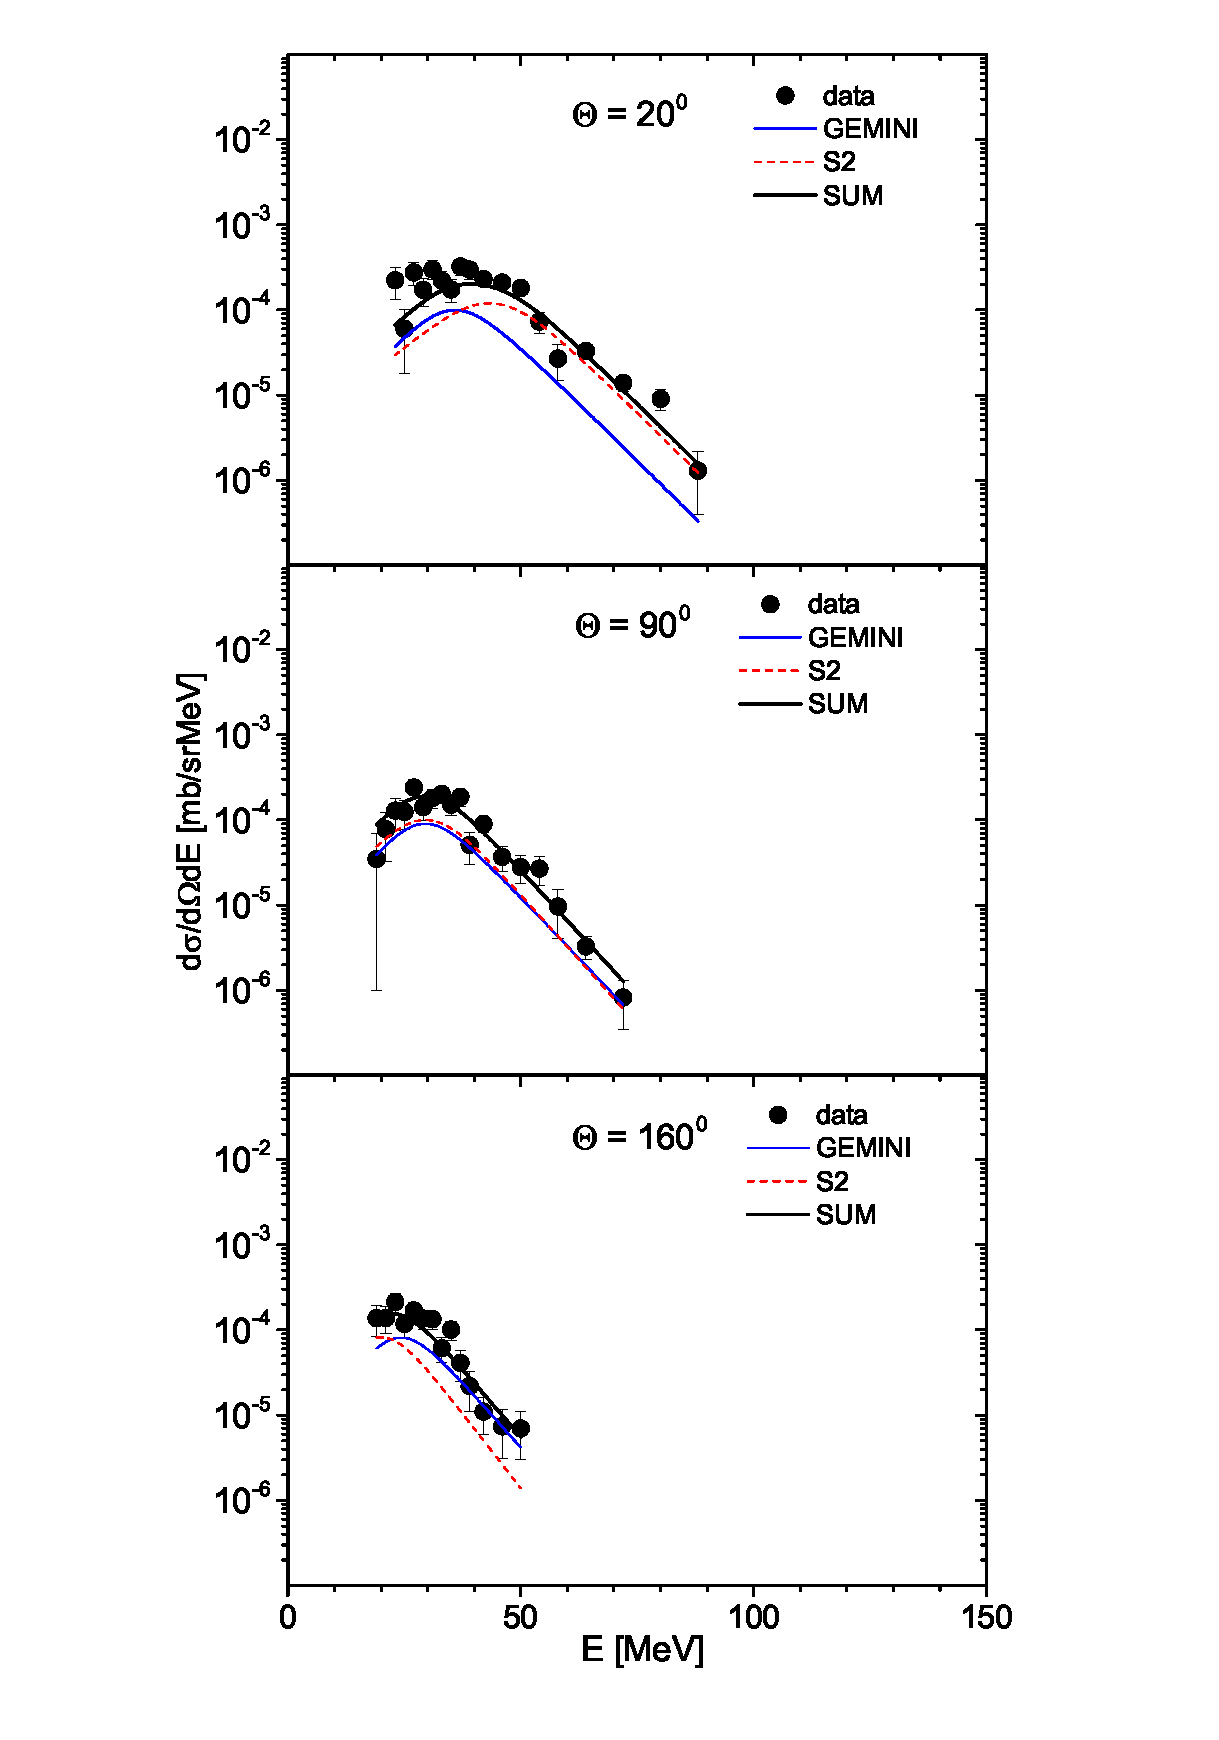
\includegraphics{18OGEMINIS2.eps}
}\\
  \caption{Experimental data (dots) and theoretical spectra for Ag(p,$^{18}$O) at three
  scattering angles: 20 degree (top panel), 90 degree (middle panel) and 120 degree (lower panel).
  The blue (solid) line represents GEMINI++ spectra, the red (dashed) line depicts contribution
  from additional moving source (S2), whereas the black (thick solid) line shows sum of both contributions.}
  \label{fig:18OGEMINIS2}
\end{figure}
%\end{figure*}
%

The procedure described above enabled us to obtain non-equilibrium
production cross section of IMF equal to the parameter $\sigma_2$ of
the slow moving source (or to the sum of $\sigma_2$ and $\sigma_3$ -
the appropriate parameters of both moving sources).  Furthermore,
sum of the equilibrium production cross section evaluated by means
of GEMINI++ and the above non-equilibrium cross section provided
value of the total production cross section.

The total cross sections due to INCL++ \cite{Mancusi14A} coupled to
GEMINI++ \cite{GEMINI++} as well as the total cross sections
obtained by fit of moving sources are presented together in Fig.
\ref{fig:SGS2S3} as a function of the atomic mass number of
ejectiles. In the lower panel of the figure the equilibrium emission
cross sections $\sigma_{\text{GEMINI}}$ are shown, in the middle
panel the non-equilibrium cross sections parameterized by slower of
the moving sources $\sigma_2$ are depicted, whereas that due to the
faster moving source $\sigma_{3}$ are shown in the upper panel of
the figure.  The cross sections for individual elements are
presented by the same symbols and are connected by lines.





%\begin{figure*}
\begin{figure}
  % Requires \usepackage{graphicx}
  \centering
  \resizebox{0.5\textwidth}{!}{%
  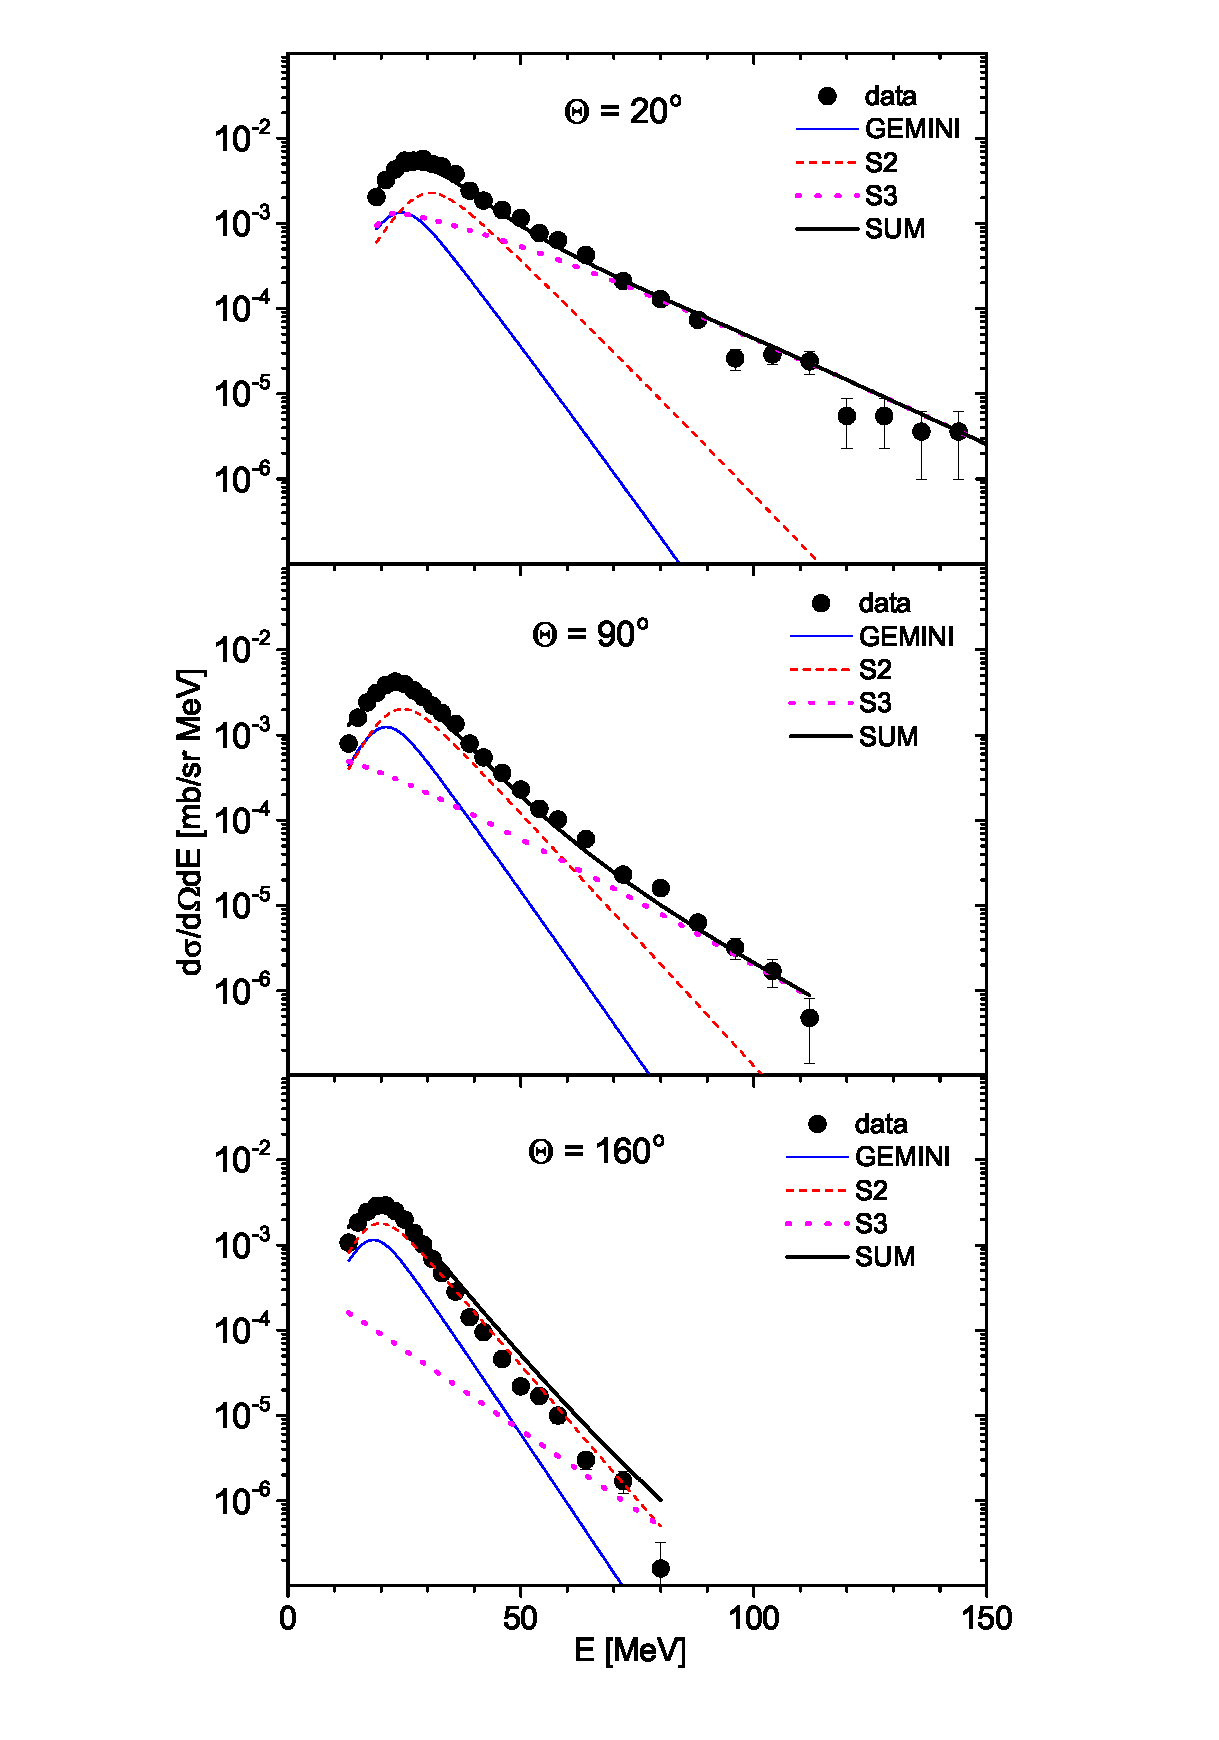
\includegraphics{9BeGEMINIS2S3.eps}
}\\
  \caption{Experimental data (dots) and theoretical spectra for Ag(p,$^9$Be) at three
  scattering angles: 20 degree (top panel), 90 degree (middle panel) and 120 degree (lower panel).
  The blue (solid) line represents GEMINI++ spectra, the red (dashed) line depicts contribution
  from slower moving source (S2), the magenta (dotted) line shows contribution of the second, faster
  source (S3) whereas the black (thick solid) line shows sum of all contributions.}
  \label{fig:9BeGEMINIS2S3}
\end{figure}
%\end{figure*}


It is clear that the cross sections decrease in average as a
function of the atomic mass number, however, this dependence of the
cross sections is non-monotonic, parabola - like  for each
individual element. It is important to note that the mass number A
of the maximal cross section  determined by the INCL+GEMINI model
for given element is not always the same as the mass number A at
which the maximal cross section of the non-equilibrium emission
appears. Furthermore, variation of the equilibrium cross sections
with the mass number seems to be more rapid than variation of the
corresponding non-equilibrium cross sections. Therefore it is quite
difficult to predict from this figure how complicated may be the
mass dependence of the ratio of non-equilibrium cross sections to
the total production cross sections
$\sigma_{\text{NEQ}}/\sigma_{\text{TOT}}$, \emph{i.e.}, to the sum
of the equilibrium and non-equilibrium cross sections.



%\begin{figure*}[H]
\begin{figure}
  % Requires \usepackage{graphicx}
  \centering
  \resizebox{0.5\textwidth}{!}{%
  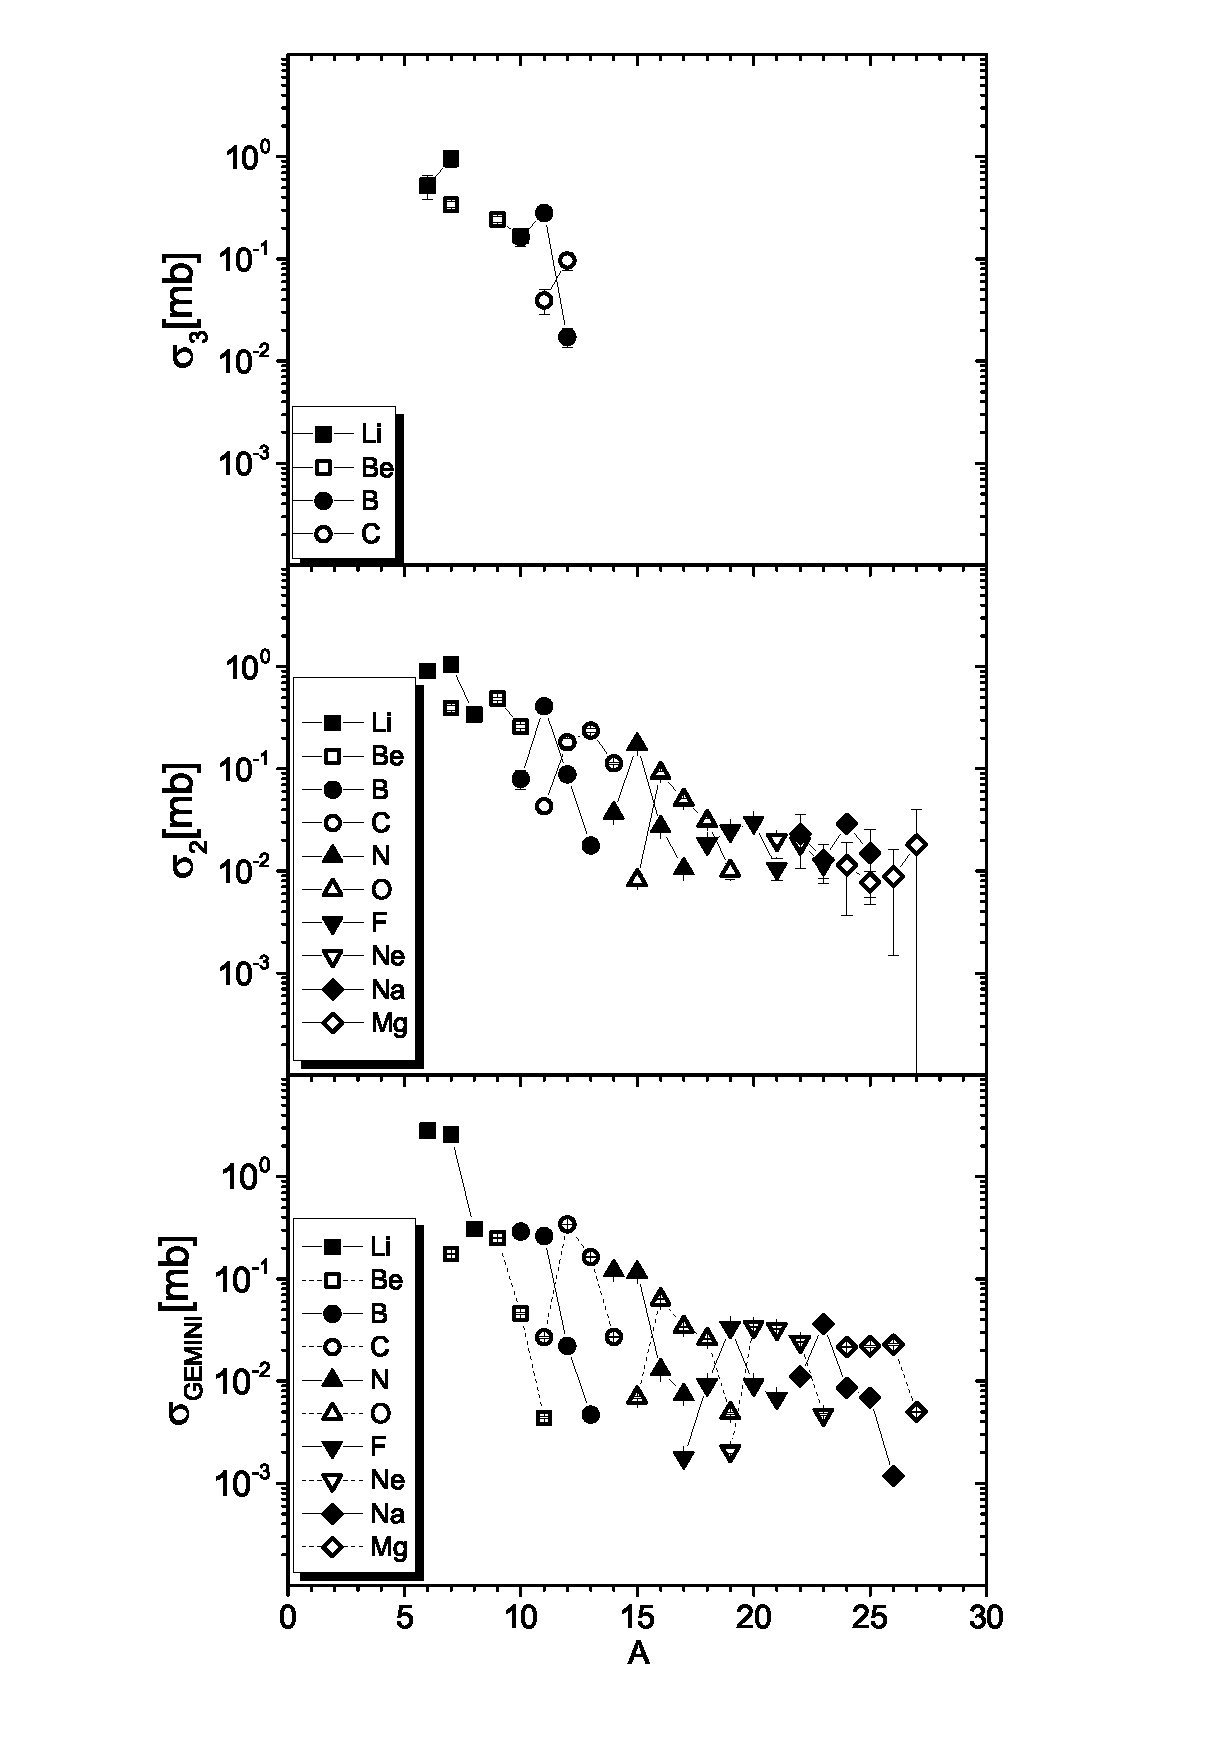
\includegraphics{SGS2S3.eps}
}\\
  \caption{Production cross sections of intermediate mass fragments evaluated by means of
  the INCL++ model coupled to the GEMINI++ one (lower panel),
  production cross sections $\sigma_2$ from the phenomenological slow moving source (middle panel) and those
  ($\sigma_3$) due to the fast moving source (upper panel).  Different elements are distinguished
  by using different symbols whereas  various isotopes
  of the same element are represented by the same symbol.}
  \label{fig:SGS2S3}
\end{figure}
%\end{figure*}
%
This quantity, which constitutes the subject of the present study is
presented in Fig. \ref{fig:RNEQtoTOTtot.eps} as a function of atomic
mass number A of produced IMF. Different symbols connected by thin
lines indicate values of the ratio for corresponding elements shown
in the description at the right hand side of the figure. The same
symbol depicts  results obtained for various isotopes of a given
element. The horizontal line placed at 0.5 value of the ratio
divides  the set of all isotopes into two groups; one with  the
ratio corresponding to the dominance of the equilibrium processes
and the second of the opposite property.



%
%
\begin{figure*}
%\begin{figure}[H]
  % Requires \usepackage{graphicx}
  \centering
  \resizebox{0.85\textwidth}{!}{%
  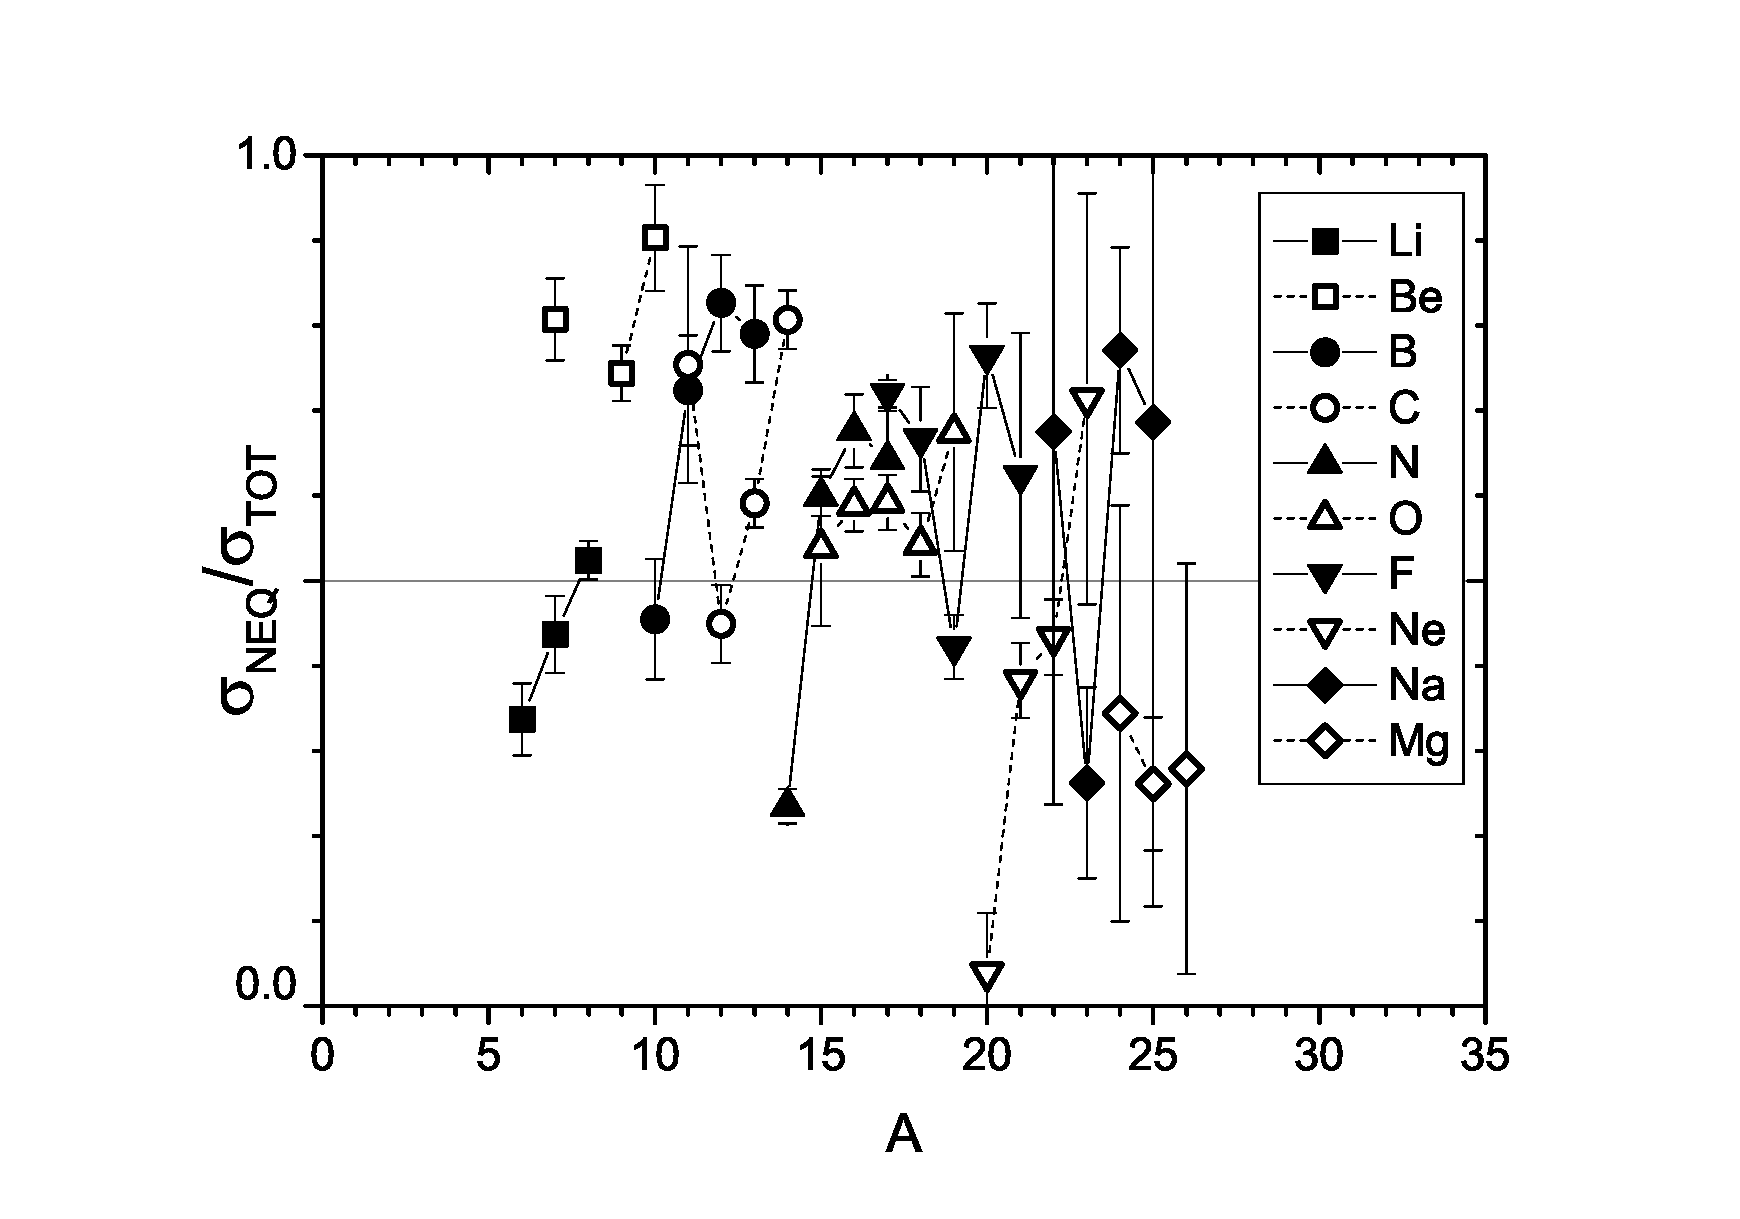
\includegraphics{RNEQtoTOTtot.eps}
}\\
  \caption{Atomic mass number A dependence of the ratio of non-equilibrium production
  cross section  to the total production cross section for intermediate mass fragments
  emerging from p+Ag collisions.
  }
  \label{fig:RNEQtoTOTtot.eps}
%\end{figure}
\end{figure*}
%





%
The following properties of the ratio of the non-equilib\-rium cross
 sections to the total cross sections may be easily
 derived from
 this figure: (i) The ratios larger than 0.5 are about 2 times more abundant
 than those smaller than 0.5.  This is true for both, small and large values
 of the atomic mass number A.
%
(ii) Values of  ratios close to 0.5 appear mainly at average
 mass number values (A $\sim$ 17) whereas those at smaller as well
 as at larger mass numbers are grouped into two separate sets.
 One set of the isotopes with the ratios smaller than 0.5
 and the second set with the ratios larger than 0.5 for the same A values.

Such a specific dependence of the ratio
$\sigma_{\text{NEQ}}/\sigma_{\text{TOT}}$ indicates that there
exists no single monotonic trend of this ratio versus mass number A
for all studied isotopes. One has to find some additional criterion
which might select the isotopes into groups behaving in the same way
when treated as a function of the mass number.

   Two specific properties of the emitted intermediate mass fragments were applied
for this purpose:

(i) the even/odd number of protons and neutrons - constituents of
the IMF, and

(ii) the third component of the isospin of the fragment T$_3 \equiv
(N-Z)/2$ representing excess (deficiency) of the number of neutrons
in respect to the number of protons. For this purpose all reaction
products were divided into 4 subgroups of definite (Z,N): (even -
even), (even - odd), (odd - even) and (odd - odd). The atomic mass
dependence of the ratio $\sigma_{\text{NEQ}}/\sigma_{\text{TOT}}$
was presented for these subgroups in separate panels of the Fig.
\ref{fig:R4eoT3}; the upper-left panel for even-even (Z,N), the
upper-right one for even-odd, \emph{etc.}, in the clockwise
direction.

It turned out that the ratio
$\sigma_{\text{NEQ}}/\sigma_{\text{TOT}}$ behaves in a very regular
way for each of these selected groups of isotopes (cf. Fig.
\ref{fig:R4eoT3}). Especially, it may be stated that this ratio
decreases in average linearly with the mass number A of emitted
fragment for even-even, even-odd and odd-even intermediate mass
fragments whereas it increases in average linearly for odd-odd
ejectiles.

Furthermore, some deviations from such a regular behaviour may be
observed for specific values of the third component of the isospin
$T_3 \equiv (N-Z)/2$ of the emitted particles. For example, two of
the four even-even ejectiles with $T_3=0$, namely $^{12}$C and
$^{20}$Ne have much smaller ratio
$\sigma_{\text{NEQ}}/\sigma_{\text{TOT}}$ than other even-even IMF
with $T_3=0$ and all $T_3=1$ particles %which very well follow a
%straight, decreasing line versus the atomic mass number A
(cf.
upper, left panel of Fig. \ref{fig:R4eoT3}).

 Second of such
deviations is the fact that all $T_3=3/2$ nuclides for even-odd and
odd-even ejectiles have larger
$\sigma_{\text{NEQ}}/\sigma_{\text{TOT}}$ ratio than that which
characterizes the $T_3=-1/2$ and $T_3=1/2$ nuclides (cf. upper-right
and lower-right panel of the Fig. \ref{fig:R4eoT3}).

The third example consists in the systematic deviation toward
smaller ratio values of $T_3=0$ ejectiles in respect to the straight
line averaging behaviour of the odd-odd group of ejectiles whereas
the IMF with $T_3=1$ deviate toward larger ratio values (cf.
lower-left panel of the Fig. \ref{fig:R4eoT3}).



\begin{figure*}
%\begin{figure}[H]
  % Requires \usepackage{graphicx}
  \centering
  \resizebox{0.85\textwidth}{!}{%
  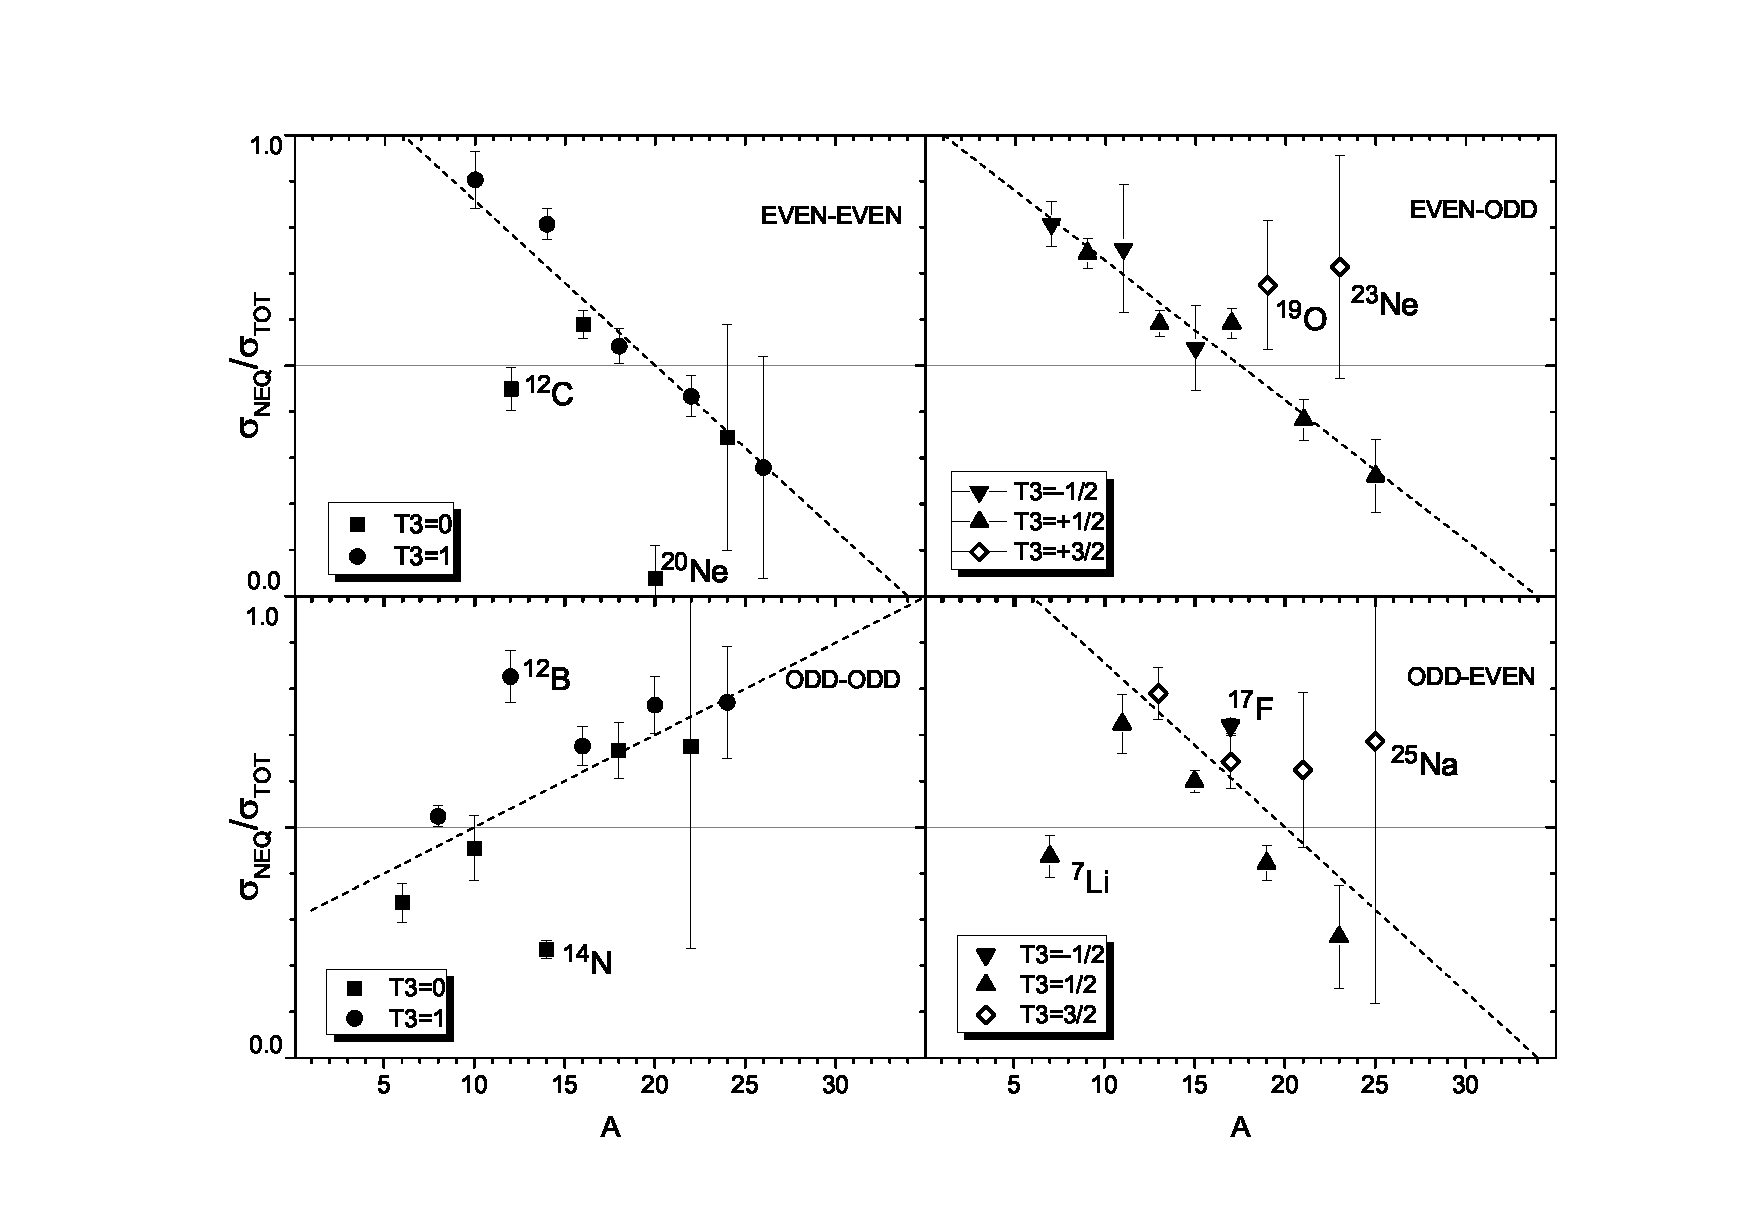
\includegraphics{R4eoT3.eps}
}\\
  \caption{Atomic mass number A dependence of the ratio of non-equilibrium production
  cross section to the total production cross section for intermediate mass fragments
  emerging from p+Ag collisions.  % at proton beam energy E$_p$=0.48 GeV.
  Left upper panel of the figure presents the results for even-even (Z,N) products
  whereas other panels
  (in clockwise direction) contain results for even-odd, odd-even and odd-odd products.
  Different symbols are attributed to values of the ratio corresponding to different values of the third
  component of the isospin $T_3=(N-Z)/A$ of ejectiles. Dashed lines are drawn to guide the eye.}
  \label{fig:R4eoT3}
%\end{figure}
\end{figure*}


While no physical model has been implied by the dependence presented
in the Fig. \ref{fig:R4eoT3}, the extremely regular behaviour
achieved in this  analysis certainly merits further consideration.




%
%
\begin{figure*}
%%\begin{figure}[H]
  % Requires \usepackage{graphicx}
  \centering
  \resizebox{0.8\textwidth}{!}{%
  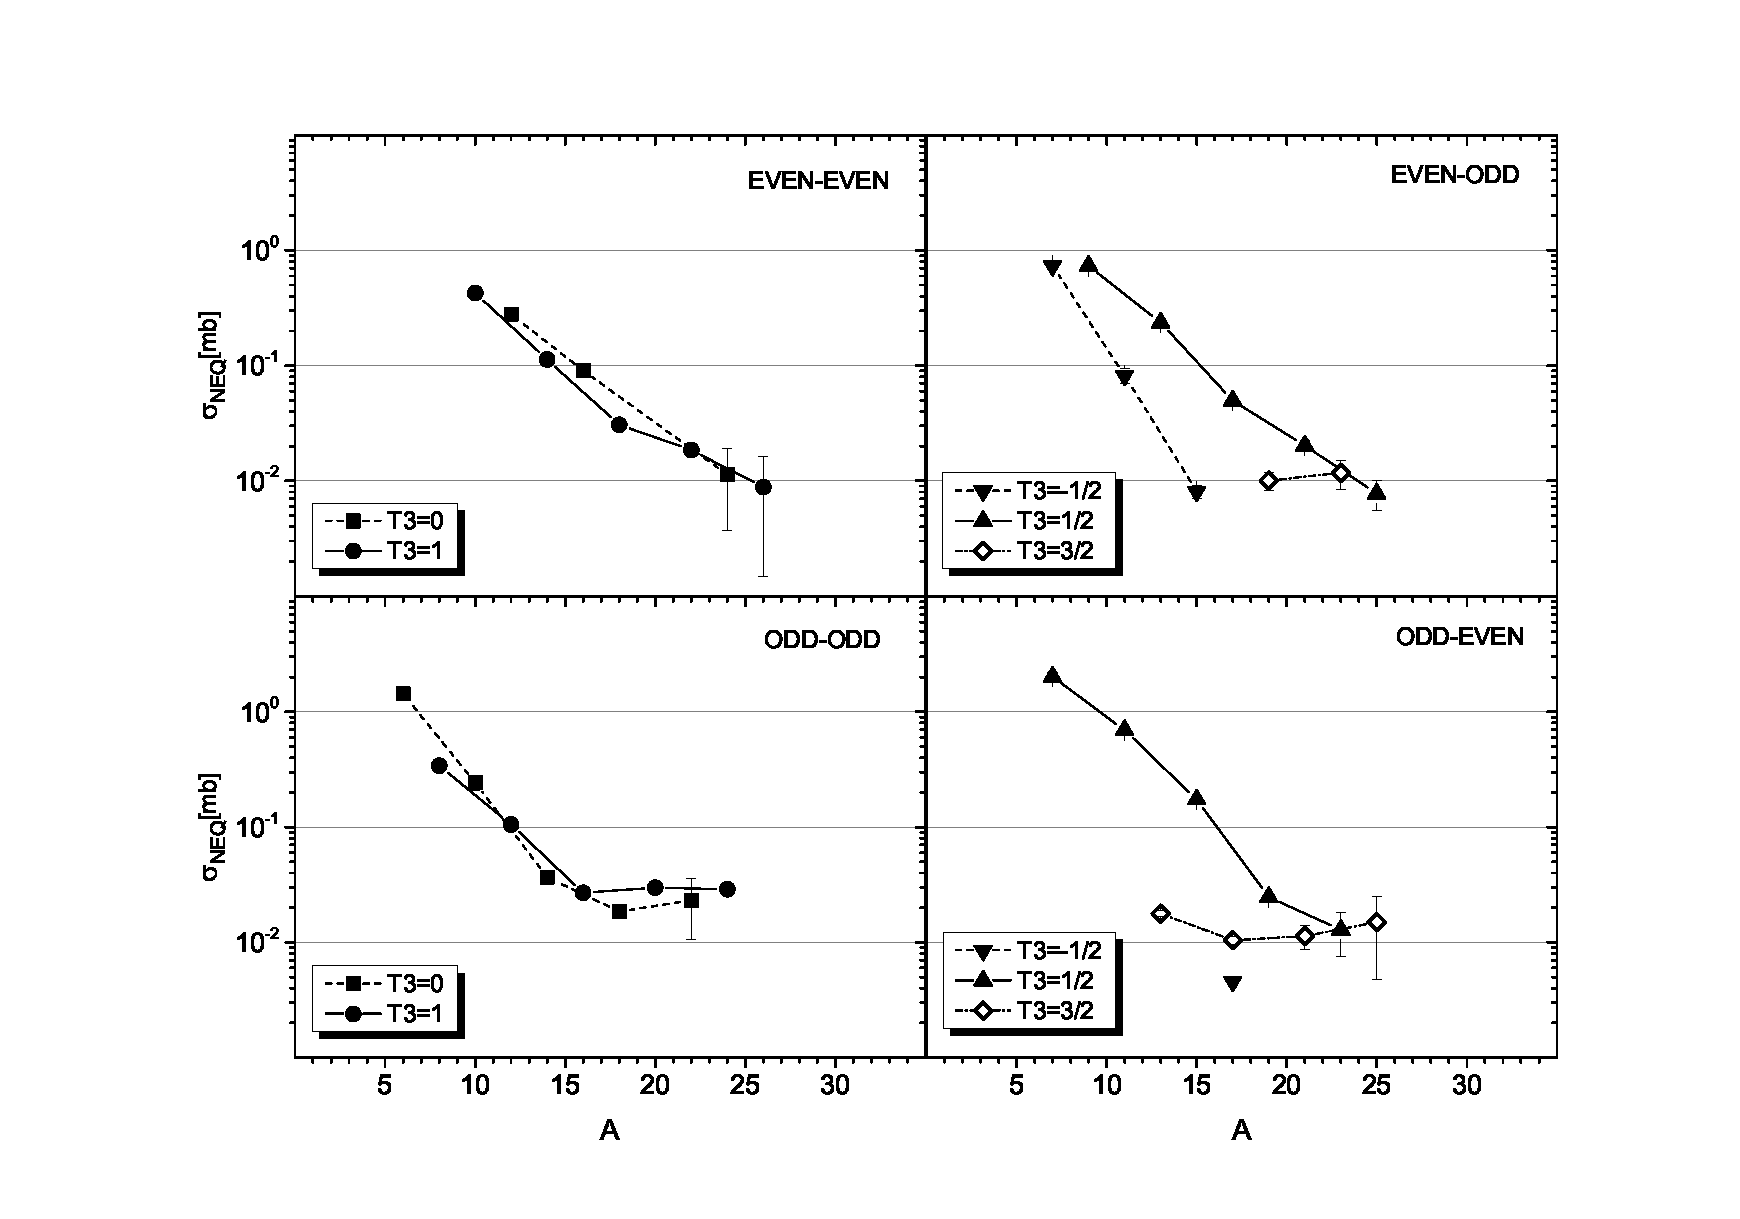
\includegraphics{S23vsAT3.eps}
}\\
  \caption{Atomic mass number dependence of  the production
  cross sections of intermediate mass fragments
  emerging due to non-equilibrium processes from p+Ag collisions.   Left upper panel
  of the figure presents the results for even-even (Z,N) products whereas other panels
  (in clockwise direction) contain results for even-odd, odd-even and odd-odd products.
  Different symbols are attributed to values of the cross sections for fragments with different values of the third
  component of the isospin $T_3=(N-Z)/A$. The solid, dashed and dot-dashed lines are drawn to guide the eye.}
  \label{fig:S23vsAT3}
%%\end{figure}
\end{figure*}


\begin{figure*}
%%\begin{figure}[H]
  % Requires \usepackage{graphicx}
  \centering
  \resizebox{0.8\textwidth}{!}{%
  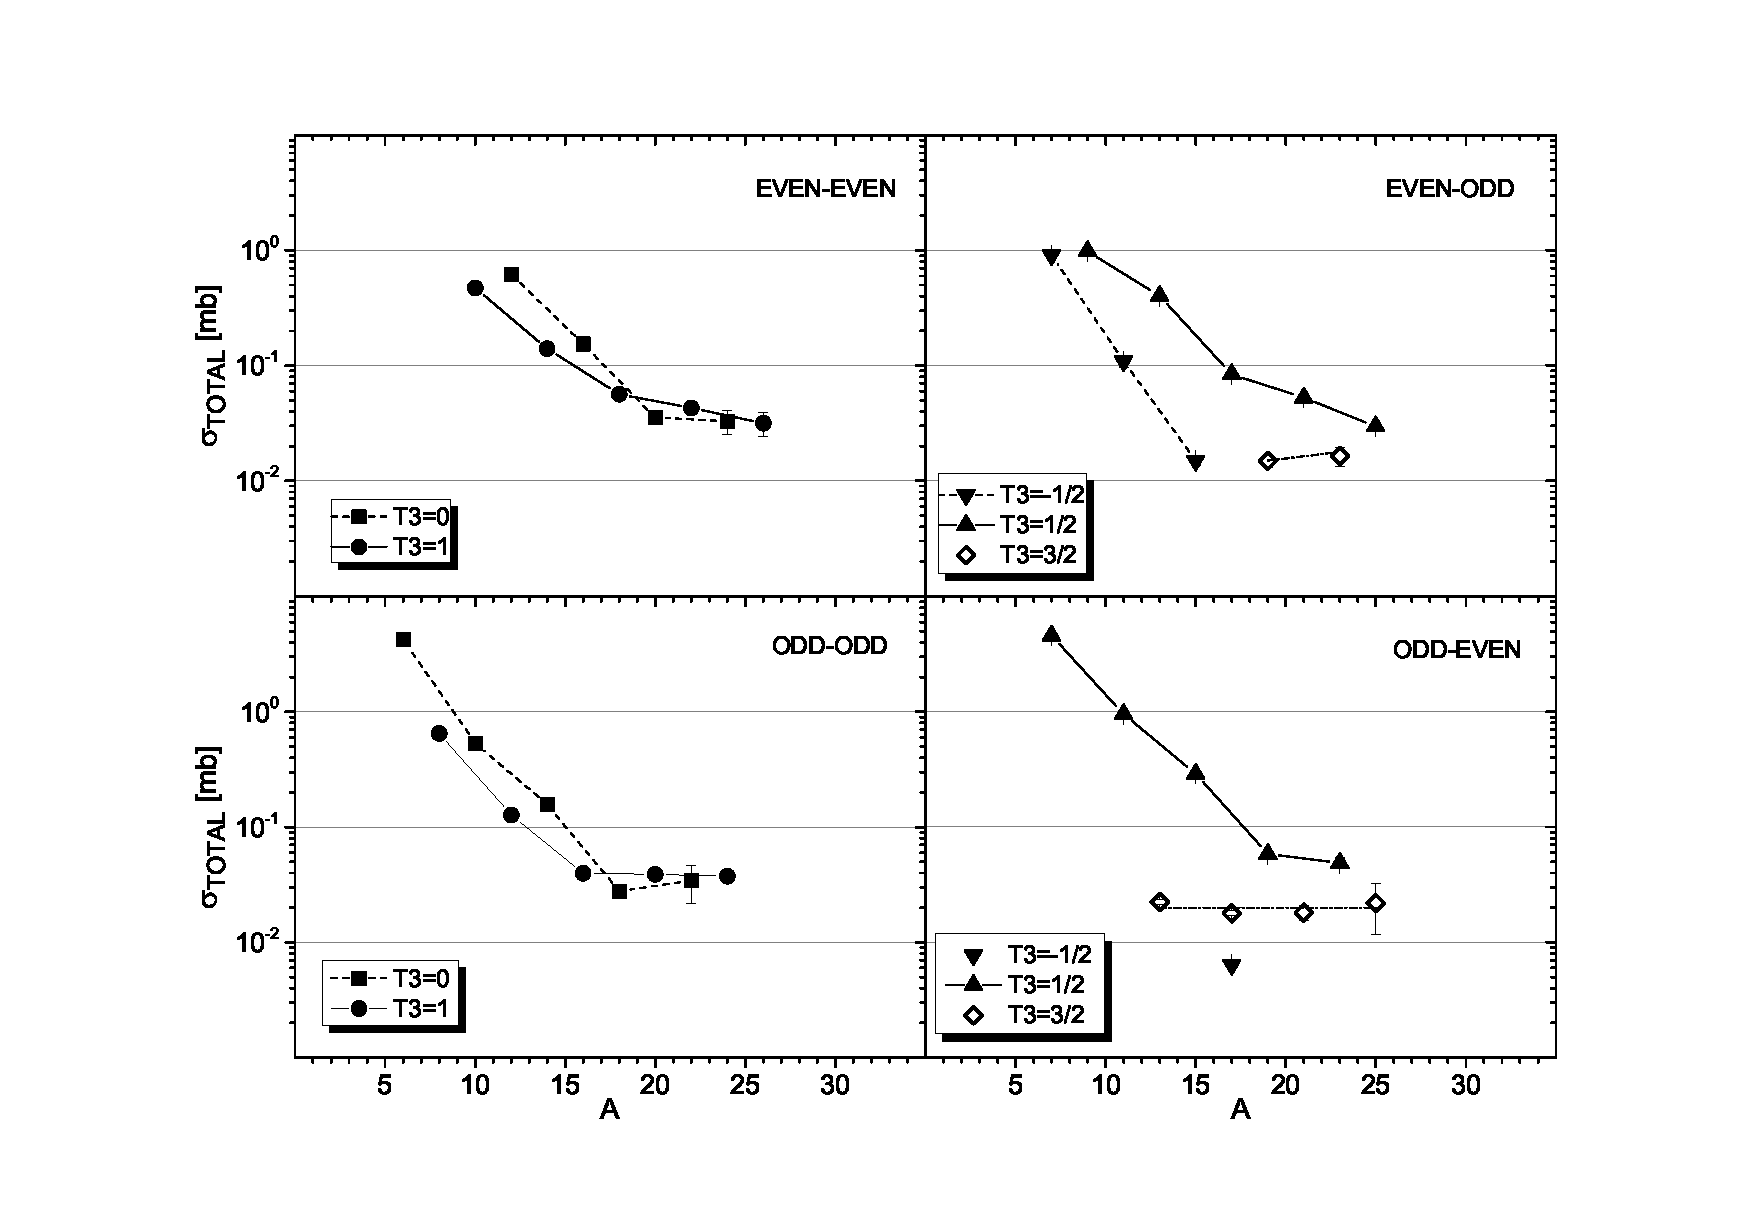
\includegraphics{TOTG23T3.eps}
}\\
  \caption{The same as in Fig. \ref{fig:S23vsAT3} but for the total
  production cross sections, \emph{i.e.}, for the sum of equilibrium and non-equilibrium production cross sections.
  The solid, dashed and dot-dashed lines are drawn to guide the eye.
%  Atomic mass dependence of  the equilibrium production
%  cross section evaluated by GEMINI++ for intermediate mass fragments
%  emerging from p+Ag collisions at proton beam energy E$_p$=0.48 GeV. Left upper panel
%  of the figure presents the results for even-even (Z,N) products whereas other panels
%  (in clockwise direction) contain results for even-odd, odd-even and odd-odd products.
%  Different symbols are attributed to values of the cross sections for fragments with different values of the third
%  component of the isospin $T_3=(N-Z)/A$. The solid, dashed and dot-dashed lines are drawn to guide the eye.
  }
  \label{fig:TOTG23T3}
%%\end{figure}
\end{figure*}





\begin{figure*}
%%\begin{figure}[H]
  % Requires \usepackage{graphicx}
  \centering
  \resizebox{0.8\textwidth}{!}{%
  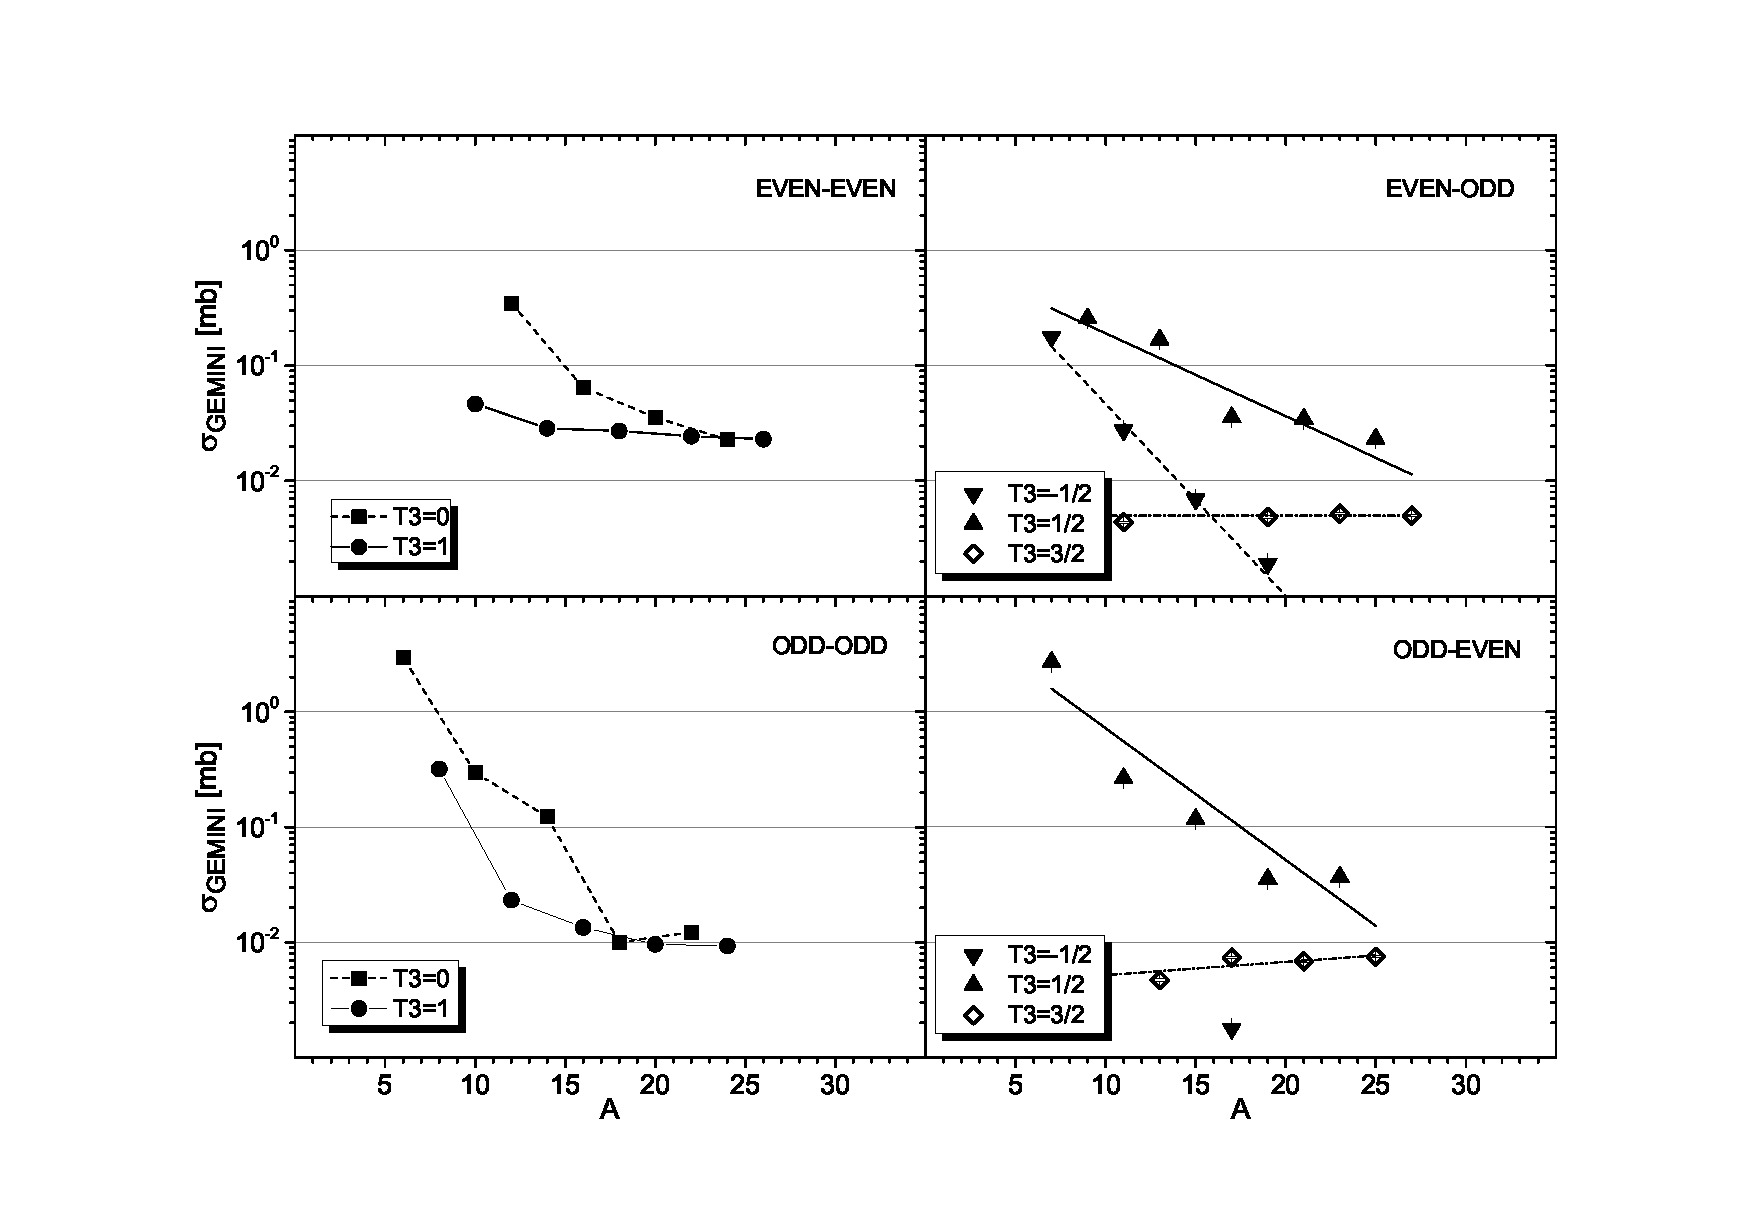
\includegraphics{GEMseparateT3.eps}
}\\
  \caption{The same as in Fig. \ref{fig:S23vsAT3} but for the equilibrium
  emission cross sections evaluated by means of the INCL++ plus GEMINI++
  models. The solid, dashed and dot-dashed lines are drawn to guide the eye.
%  Atomic mass dependence of  the equilibrium production
%  cross section evaluated by GEMINI++ for intermediate mass fragments
%  emerging from p+Ag collisions at proton beam energy E$_p$=0.48 GeV. Left upper panel
%  of the figure presents the results for even-even (Z,N) products whereas other panels
%  (in clockwise direction) contain results for even-odd, odd-even and odd-odd products.
%  Different symbols are attributed to values of the cross sections for fragments with different values of the third
%  component of the isospin $T_3=(N-Z)/A$. The solid, dashed and dot-dashed lines are drawn to guide the eye.
  }
  \label{fig:GEMseparateT3}
%%\end{figure}
\end{figure*}
 %
\section{Hybrid (phenomenological+microscopic) approach to describe the double-differential cross sections features of total cross sections – odd-even staggering}
\section{Comparison of models and conclusion about their limitation}
\chapter{Odd-even staggering of total production cross-section in spallation reactions}\label{chapter:7}
 \section{Determination of non-equilibrium cross-section of IMF in p + Ag reaction at 480 MeV}
\section{Dependence of this component on third component of isospin}
\chapter{Summary}
\section{Validation of total cross-section}
	The following analyzes were performed using the p+Ag and p+ 136 Xe
	data:
	Investigation of the quality of reproduction of the isotopic production cross sections for emission of different isotopes of the Li, Be, ... Ba nuclei from collisions of 1 GeV protons with 136 Xe by combination of two models: The INCL++ model describing fast, non-equilibrium phase of the collisions coupled to ABLA07,GEM,GEMINI and SMM models which were used to reproduce the second phase of the process, i.e. -emission of products from equilibrated remnant of the first stage of the processes.(This is the content of published paper \cite{singh2018predictive})
	\section{Validation of differential cross-section for IMF and heavy products}
	Analysis of angular distributions for double differential cross sections $d\sigma/d\Omega dE$ for intermediate mass fragments (isotopes of Li, Be, ... Mg elements) emitted from p+Ag reaction at E p =0.48 GeV with the aim to extract:
	\begin{itemize}
		\item Contribution of the non-equilibrium processes to the reaction, 
		\item Dependence of the isotopic total cross sections of these reactions on the izospin degree of freedom.
	\end{itemize}
	
	(This is the content of [UNPUB] paper prepared for publication in EPJA but
	rejected by referees)
	Investigation of the odd-even staggering in the yields of IMFs from the above reac-
	tion, i.e. p+Ag collisions at E p =0.48 GeV with the aim to study a possibility to
	validate models of the spallation reactions using this degree of freedom. (This is
	the content of Acta Phy)
	\section{LCP data analysis and validation of different models}
	Determination of differential cross sections $d\sigma/d\Omega dE$ for emission of Hydrogen isotopes as well as pions ( $\pi^+$ and $\pi^-$ ) using raw data stored event-by-event from collisions of protons with Nb nuclei at E p =3.5 GeV in HADES collaboration experiment performed at GSI in Sep 2008. Theoretical analysis of these data by means of following theoretical models like INCL++ ,BUU, UrQMD, JAM.
	The above investigations of HADES data were performed with the aim to shed light on the first, non-equilibrium part of the proton-nucleus collisions whereas the analysis of the literature data for p+Ag and p+ 136 Xe gave a chance to obtain information on
	the mechanism of the second, slow stage of the collision process which appears after equilibration of the excited remnant of the target nucleus.
\printbibliography
\end{document}
% \appendix
% \chapter{Appendix Title}
% \input{chapters/appendix}